% Additive source-synchronised revision. Build and inspection receipts are separate.
\documentclass[12pt,a4paper]{article}
\usepackage{fontspec}
\setmainfont{Liberation Serif}
\setsansfont{Liberation Sans}
\setmonofont{DejaVu Sans Mono}[Scale=0.85]
\usepackage[left=30mm,right=25mm,top=25mm,bottom=25mm]{geometry}
\usepackage{amsmath,amssymb,amsthm}
\usepackage{graphicx}
\usepackage{array,booktabs,longtable,tabularx,xltabular}
\usepackage{caption}
\usepackage{algorithm}
\usepackage{fvextra}
\usepackage{xurl}
\usepackage{setspace,ragged2e,placeins,needspace}
\usepackage[hidelinks,unicode]{hyperref}
\newtheorem{proposition}{Proposition}
\renewcommand{\theHtable}{\thesection.\arabic{table}}
\newcolumntype{Y}{>{\RaggedRight\arraybackslash\hspace{0pt}}X}
\setcounter{secnumdepth}{2}
\setcounter{tocdepth}{2}
\captionsetup{font=small,labelfont=bf,justification=raggedright,singlelinecheck=false}
\setlength{\parindent}{0pt}
\setlength{\parskip}{0.45em}
\setlength{\emergencystretch}{2em}
\newcommand{\appendixsection}[2]{%
  \clearpage\refstepcounter{section}%
  \section*{Appendix \thesection. #2}%
  \addcontentsline{toc}{section}{Appendix \thesection. #2}%
  \label{#1}\setcounter{table}{0}%
}
\begin{document}
\pagenumbering{arabic}
\thispagestyle{empty}
\begin{center}
\vspace*{12mm}
{\Large\bfseries TrafficTwin: Admission and Dispatch Semantics in Vehicular Edge Computing under a Frozen MAPPO Policy\par}
\vspace{18mm}
{\large S M Abdulla Al Mamun\par}
\vspace{12mm}
{\large The University of Manchester\par}
\vspace{8mm}
Master's dissertation\par
2026\par
\vspace{12mm}
Supervisor: Dr Sandra Sampaio\par
\end{center}
\vfill
\begin{tabular}{@{}ll@{}}
Award wording: & \rule{95mm}{0.3pt}\\[9pt]
Faculty and School: & \rule{95mm}{0.3pt}\\[9pt]
Student ID: & \rule{95mm}{0.3pt}
\end{tabular}
\clearpage
\tableofcontents
\vfill\noindent\textbf{Word count: 8,987.} References, appendices, captions and front matter
excluded; Abstract, table text and pseudocode included. The counting receipt records
tokenisation.\par
\clearpage
{\small\singlespacing
\listoffigures
\listoftables
}
\clearpage
\section*{Abbreviations}
\addcontentsline{toc}{section}{Abbreviations}
\begin{tabularx}{\textwidth}{@{}lX@{}}
CI & Confidence interval\\
CLI & Command-line interface\\
CPU & Central processing unit\\
DRL & Deep reinforcement learning\\
E0--E2d & Historical validation, scoping and dispatch study stages\\
E3 & Separate dynamic-resource campaign, not executed\\
EV & Electric vehicle\\
ITS & Intelligent transportation systems\\
JAX & Array-computing and automatic-differentiation framework\\
MAPPO & Multi-agent proximal policy optimisation\\
PPO & Proximal policy optimisation\\
RQ & Research question\\
RSU & Roadside unit\\
SoC & State of charge\\
SUMO & Simulation of Urban MObility\\
V2I / V2V & Vehicle-to-infrastructure / vehicle-to-vehicle\\
VEC & Vehicular edge computing\\
\end{tabularx}
\clearpage
\onehalfspacing\RaggedRight
% BEGIN SOURCE BLOCK 002 heading
\section*{Abstract}\addcontentsline{toc}{section}{Abstract}\phantomsection\label{sec:abstract}
% END SOURCE BLOCK 002

% BEGIN SOURCE BLOCK 003 paragraph
A vehicle's strongest radio link can lead to a busy computing server, and admitting its task does not guarantee a result before the deadline. TrafficTwin investigates how infrastructure scheduling changes offered-task deadline attainment under a fixed, pretrained vehicle offloading policy. The comparison separates radio ingress, execution placement, admission and workload reservation.
% END SOURCE BLOCK 003

% BEGIN SOURCE BLOCK 004 paragraph
Common-target least-workload placement underperformed execution at ingress, while causal per-task placement improved it. This reversal appeared in an adaptive incident study and a separate four-draw morning replication that excluded its inspected pilot. A later confirmation completed 32 evaluations across eight fresh joint fleet/evaluator-seed blocks. Per-task minus ingress was +4.137 percentage points; common-target minus ingress was \ensuremath{-}3.504. Per-task also exceeded causal cyclic spreading by +0.631 points, with a Bonferroni simultaneous 95\% interval of [+0.511, +0.750]. All actions matched, although feedback was permitted and small observation/logit differences occurred in one block.
% END SOURCE BLOCK 004

% BEGIN SOURCE BLOCK 005 paragraph
Retrospective analysis explains recurring common destinations through shared assignment, queue clearing and deterministic ties. The exact-model proof establishes when fixed-target reconciliation reproduces sequential admission; rounding limits its application to executable arithmetic. Original morning task accounting locates most gains in reduced gate rejection, while retaining individual losses. Separate CPU fixtures show that workload-aware targeting costs more than cyclic spreading, despite outperforming the common-target implementation in scheduler-only timing.
% END SOURCE BLOCK 005

% BEGIN SOURCE BLOCK 006 paragraph
The findings support a bounded benefit from workload awareness beyond spreading. One actor, the same morning trace for confirmation, global service-work information and aggregate timing restrict generalisation and physical interpretation. Historical capacity findings separately retain inconclusive statistics and unresolved scoring uncertainty; the later gate-enabled results do not resolve that gap.
% END SOURCE BLOCK 006


\clearpage
\section*{Declaration}
\addcontentsline{toc}{section}{Declaration}
\textbf{Assistance and attribution.} I designed this study and every evaluation experiment reported here, and I am responsible for the analysis and its interpretation. The software was developed by me with generative-AI assistance: Codex and ChatGPT produced code, campaign tooling and draft text to my specification, which I reviewed and in many cases rewrote before use. Randy Prasetia Putra supplied the MAPPO actor, the vec\_env environment and evaluator, and the accounting repair of 5 August 2026. Dr Sandra Sampaio suggested the report-age levels used in Section~\ref{sec:2.7}. Automated build and validation receipts identify the checks that were executed; my own verification of the results is recorded in the contribution statement (Section~\ref{sec:3.7}).

\medskip
\textbf{Candidate declaration to be signed.} The contribution statement and declared assistance
accurately describe the work submitted, and all non-original material is acknowledged.\par
\medskip
Prior submission for another qualification (select and complete):\par
$\square$ None.\qquad $\square$ Portions specified below.\par
\rule{\textwidth}{0.3pt}\par
\rule{\textwidth}{0.3pt}\par
\bigskip
Signature: \rule{60mm}{0.3pt}\qquad Date: \rule{25mm}{0.3pt}
\clearpage
\section*{Copyright and intellectual property}
\addcontentsline{toc}{section}{Copyright and intellectual property}
Original text, third-party material, source code and research inputs retain their respective
rights and applicable University arrangements. Access to a private repository or research
dataset does not grant unrestricted redistribution rights. Reuse must respect the relevant
licences, permissions and contributor acknowledgements. The software, actor, traffic inputs and
evidence records are separately identified so that their ownership is not conflated with
authorship of this report.
\clearpage
\section*{Acknowledgements}
\addcontentsline{toc}{section}{Acknowledgements}
I thank Dr Sandra Sampaio for supervising this project and suggesting the report-age levels. I thank Randy Prasetia Putra for supplying the MAPPO actor, the vec\_env environment and evaluator, and the accounting repair. Automated assistance is disclosed in the Declaration.
\clearpage

% BEGIN SOURCE BLOCK 007 heading
\section{Introduction}\label{sec:1}
% END SOURCE BLOCK 007

\FloatBarrier
% BEGIN SOURCE BLOCK 008 heading
\subsection{Problem and motivation}\label{sec:1.1}
% END SOURCE BLOCK 008

% BEGIN SOURCE BLOCK 009 paragraph
Vehicular edge computing concerns where a vehicle's computational tasks should run and whether their results can return before a deadline. A task may execute locally, use a neighbouring vehicle through vehicle-to-vehicle communication (V2V), or enter roadside infrastructure through vehicle-to-infrastructure communication (V2I). A roadside unit (RSU) combines a radio access point with a simulated computing server in this study. Offloading therefore couples communication conditions with the work already waiting for computation \cite{ref1}.
% END SOURCE BLOCK 009

% BEGIN SOURCE BLOCK 010 paragraph
Deadline attainment matters because a computed answer has value only within the time window in which the application can use it. Moving computation away from a vehicle can provide access to additional resources, but it also adds transmission and waiting. A scheduling decision must therefore account for the path to an answer, rather than regard successful offloading as the endpoint. The mobile-edge literature frames this as joint communication and computation management \cite{ref1}. I use offered-task deadline attainment to make that distinction explicit: the question is how much of the requested work receives a timely result.
% END SOURCE BLOCK 010

% BEGIN SOURCE BLOCK 011 paragraph
Vehicle mobility makes this question especially relevant. Radio conditions and the vehicles present around an RSU can change while previously admitted work still occupies its server. A good connection at the instant of offloading does not establish that the destination has spare computing service. Research on heterogeneous vehicular edge computing accordingly considers communication and resource allocation together with stringent latency requirements \cite{ref18}. In this dissertation, those concerns motivate a controlled question about infrastructure decisions under fixed vehicle-policy weights, rather than a claim to reproduce all the timing requirements of an operational transport application.
% END SOURCE BLOCK 011

% BEGIN SOURCE BLOCK 012 paragraph
The Manchester scenarios give the comparison a concrete traffic setting. I use saved SUMO working-day and incident-model traces to expose the same scheduling rules to different scenario conditions. The traces supply simulated vehicle movement; their role is to define repeatable inputs, not to establish live performance on Manchester roads. An operator must decide whether to retain ingress execution, distribute work or alter admission, accounting for coordination cost and available service.
% END SOURCE BLOCK 012

% BEGIN SOURCE BLOCK 013 paragraph
The surrounding research also includes RSU-to-RSU cooperation \cite{ref24} and task inference across vehicle, RSU and edge resources \cite{ref25}. These identify a wider setting in which execution location matters; I do not transfer their performance claims to TrafficTwin. My narrower comparison makes an infrastructure choice inspectable while leaving the upstream actor fixed. This scope supports a precise distinction between accepting work, distributing it and completing it before its deadline. It also makes an unfavourable result informative: a scheduler can spread nominal demand or use a least-workload label without improving the proportion of all offered tasks that finish in time.
% END SOURCE BLOCK 013

% BEGIN SOURCE BLOCK 014 paragraph
The \textbf{ingress RSU} provides the strongest simulated radio link; \textbf{execution placement} selects the computing server. Another RSU may offer less waiting at a coordination cost. Figure~\ref{fig:1} separates the vehicle's offloading mode from infrastructure execution and admission \hyperref[source-s4]{[S4]}.
% END SOURCE BLOCK 014

% BEGIN SOURCE BLOCK 015 paragraph
Admission does not guarantee timely completion. The backlog gate excludes the arriving task's own service and transmission time. I retain rejected tasks in the offered denominator so selective admission cannot conceal failures.
% END SOURCE BLOCK 015

% BEGIN SOURCE BLOCK 016 paragraph
I froze the supplied multi-agent proximal policy optimisation (MAPPO) actor's weights; matched inputs and action checks distinguish infrastructure effects from retraining and observation feedback.
% END SOURCE BLOCK 016

% BEGIN SOURCE BLOCK 017 paragraph
The programme progressed from accounting and capacity to opposite ingress rankings for two least-workload implementations, distinguished by target timing, reservations and admission \hyperref[source-s0]{[S0]}--\hyperref[source-s4]{[S4]}.
% END SOURCE BLOCK 017

% BEGIN SOURCE BLOCK 018 figure
\begin{figure}[htbp]
\centering
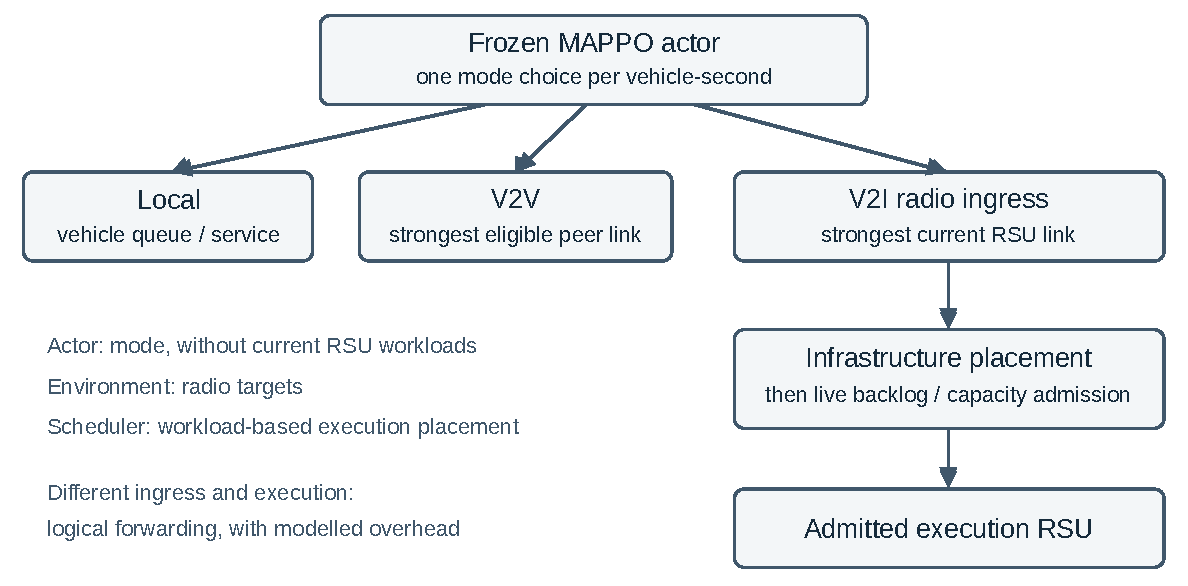
\includegraphics[width=\linewidth,height=.57\textheight,keepaspectratio]{assets/architecture.pdf}
\caption[Experimental responsibility boundaries]{Experimental responsibility boundaries. Only admitted V2I work enters the selected execution queue; logical forwarding applies when ingress and execution differ. Resource scaling is outside the completed comparison \hyperref[source-s11]{[S11]}. Reading: follow the separation between vehicle mode choice, radio ingress and infrastructure execution placement.}\label{fig:1}
\end{figure}
% END SOURCE BLOCK 018

% BEGIN SOURCE BLOCK 019 paragraph
Communication and computation jointly determine whether an offloaded task returns in time \cite{ref1}, \cite{ref18}.
% END SOURCE BLOCK 019

% BEGIN SOURCE BLOCK 020 paragraph
Figure~\ref{fig:2} shows the authenticated morning RSU layout in local trace metres, not deployed Manchester equipment. Incident coordinates are absent from the compact evidence and are not invented. Each comparison preserves its scenario's trace and layout (Table~\ref{tab:2}).
% END SOURCE BLOCK 020

% BEGIN SOURCE BLOCK 021 figure
\begin{figure}[htbp]
\centering
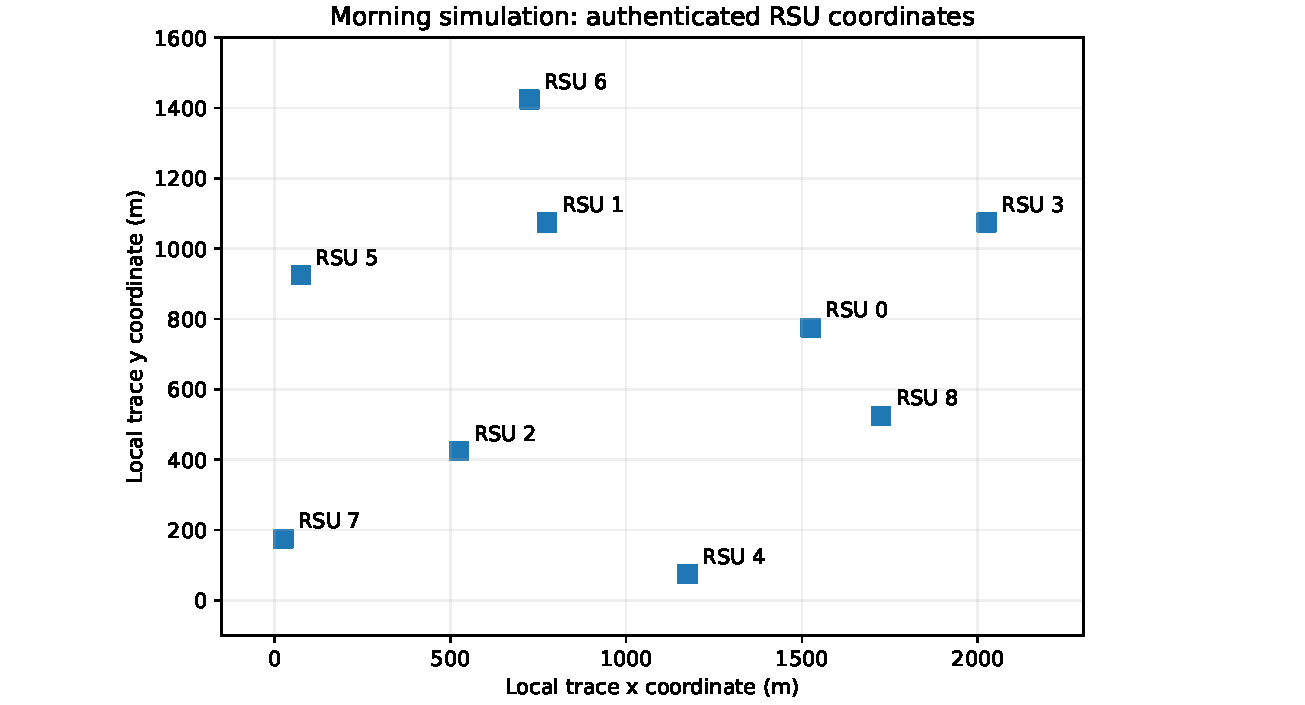
\includegraphics[width=\linewidth,height=.57\textheight,keepaspectratio]{assets/morning_rsu_layout.pdf}
\caption[Morning RSU coordinates]{Morning trace RSU positions copied from the canonical input-validation record, with original zero-based indices. The incident trace contains ten RSUs; its positions are not reconstructed here. Local network coordinates are not latitude/longitude or a verified street-map projection \hyperref[source-s8]{[S8]}. Reading: the nine morning locations are spatial inputs, whereas the dispatch comparisons change task destinations without moving these RSUs.}\label{fig:2}
\end{figure}
% END SOURCE BLOCK 021

\FloatBarrier
% BEGIN SOURCE BLOCK 022 heading
\subsection{Related work and the position of this study}\label{sec:1.2}
% END SOURCE BLOCK 022

% BEGIN SOURCE BLOCK 023 paragraph
With RL supplying the upstream policy, the closest comparison is parallel-server dispatch: what information estimates waiting time, and when an assignment changes it.
% END SOURCE BLOCK 023

% BEGIN SOURCE BLOCK 024 paragraph
\textbf{Queue count and remaining work.} With heterogeneous tasks, shortest queue and shortest workload can select different servers. Harchol-Balter, Crovella and Murta compare least-work-remaining, random, round-robin and size-based assignment under immediate assignment, identical hosts, non-preemptive first-come-first-served service and Poisson arrivals. Preferred policies depend on task-size variability \cite{ref2}. TrafficTwin's \path{jsq} compares service milliseconds; a separate task count limits admission. Neither the label nor balanced allocation establishes optimality.
% END SOURCE BLOCK 024

% BEGIN SOURCE BLOCK 025 paragraph
\textbf{Batch decisions and reservations.} Sparrow pools probes, spreads tasks and binds queued reservations when workers become ready. It identifies queue-count prediction errors and competing schedulers' apparently idle workers \cite{ref9}. Information sharing across a batch differs from committing assignments to one unchanged destination. TrafficTwin tests the latter and assumes immediate service-work information and acknowledgement, unlike Sparrow's worker-triggered binding.
% END SOURCE BLOCK 025

% BEGIN SOURCE BLOCK 026 paragraph
Ying, Srikant and Kang make the reservation distinction especially explicit: batch-filling samples queue counts, assigns tasks one by one and updates the chosen queue after each assignment. Their analysis assumes identical servers, exponential service, Poisson batch arrivals and random ties \cite{ref13}. This is close prior art for sequential within-batch updates. The evaluator also implements a power-of-two-choices variant (\path{dla_p2c}) that was not evaluated here. Although the evaluator comments mention their batch-filling work, its common-target reconciliation does not implement that destination rule. TrafficTwin's causal change is therefore an adaptation of established dispatch semantics, evaluated with workload information and deadline admission, rather than a novel batching principle.
% END SOURCE BLOCK 026

% BEGIN SOURCE BLOCK 027 paragraph
\textbf{Local information and common destinations.} Vargaftik, Keslassy and Orda's Local Shortest Queue (LSQ) policies use possibly outdated queue counts. A dispatcher can send a slot's jobs to one locally shortest queue with random ties, update estimates for sent work and refresh entries through communication. Stability requires arrival/service assumptions and bounded expected estimation error \cite{ref10}. TrafficTwin instead uses service work, deterministic ties, a backlog gate, five ordered slots and one-second draining; LSQ's stability and communication results do not establish its finite-horizon deadline performance.
% END SOURCE BLOCK 027

% BEGIN SOURCE BLOCK 028 paragraph
\textbf{Admission and useful completion.} Niño-Mora jointly studies admission and routing to heterogeneous multiserver queues, with separate costs for rejection and admitted deadline misses. Poisson arrivals, exponential service, soft deadlines and state-dependent index policies differ from TrafficTwin's inherited backlog filter \cite{ref11}. I preserve that filter to isolate placement and count success over all offers: reject-all scores zero. Neither the denominator nor the admission principle is new.
% END SOURCE BLOCK 028

% BEGIN SOURCE BLOCK 029 paragraph
Differences in arrival processes, objectives and resource models prevent treating published performance scores as controlled benchmarks. Table~\ref{tab:1} instead compares the operational mechanisms relevant to TrafficTwin.
% END SOURCE BLOCK 029

% BEGIN SOURCE BLOCK 030 table
\begingroup
\singlespacing\footnotesize\setlength{\tabcolsep}{3pt}
\begin{xltabular}{\textwidth}{@{}YYYY@{}}
\caption[Closest-work comparison]{Closest-work comparison. ``Work'' means remaining service demand; ``count'' means queued jobs. TrafficTwin rows describe the frozen implementation, not a scheduling-family definition. Reading: compare decision semantics and evidence boundaries rather than equating methods by their scheduling labels.}\label{tab:1} \\
\toprule
Work / decision layer and arrivals & Information and update semantics & Admission / objective & Relationship to TrafficTwin \\
\midrule\endfirsthead
\toprule
Work / decision layer and arrivals & Information and update semantics & Admission / objective & Relationship to TrafficTwin \\
\midrule\endhead
\bottomrule\endfoot
Harchol-Balter et al. \cite{ref2}: dispatch each arrival & Known service work; central per-arrival choice & Mean waiting time; size-normalised waiting & Closest least-workload comparator; no vehicular gate \\
Sparrow \cite{ref9}: parallel-job task placement & Sampled workers; queued reservations; worker replies bind tasks & Job response time; placement constraints & Batch spreading differs from one common destination; communication is explicit \\
Ying et al. \cite{ref13}: tasks within an arriving batch & Sampled counts; update after each assignment; random ties & Delay and sampling cost & Closest within-batch update rule; no deadline gate \\
LSQ \cite{ref10}: dispatcher batch per time slot & Local queue counts; own-assignment increments and sampled/pushed updates & Stability under specified assumptions & Common routing is established; random ties and distributed estimates differ \\
Niño-Mora \cite{ref11}: joint admission/routing per arrival & Queue counts and model-based indices & Rejection and deadline-miss costs & Supports joint evaluation, not the inherited backlog predicate \\
TrafficTwin common-target: one choice per substep & Global service work; vectorised candidate offsets and three reconciliations & Backlog gate plus finite task limit & Frozen vehicle policy; instantaneous logical forwarding \\
TrafficTwin per-task: ordered candidate scan & Global service work; actual admitted work reserved immediately & Same predicate and limit, causal admission & Tested implementation change; global information is assumed \\
\end{xltabular}
\endgroup
% END SOURCE BLOCK 030

% BEGIN SOURCE BLOCK 031 paragraph
\textbf{Attribution and simulation validity.} Sargent distinguishes model verification from operational validation \cite{ref12}. Conservation and replay checks establish the former; physical RSU/network measurements would be needed for deployment claims. SUMO trajectories \cite{ref8} do not independently validate the coupled radio/computing model.
% END SOURCE BLOCK 031

% BEGIN SOURCE BLOCK 032 paragraph
PPO and MAPPO identify the reused actor's provenance \cite{ref3}, \cite{ref4}. Henderson et al., Agarwal et al. and Gorsane et al. motivate exposing implementation choices and finite-run uncertainty \cite{ref5}, \cite{ref6}, \cite{ref7}. TrafficTwin checks action equality empirically and uses draws or joint-seed blocks, not tasks, as replications.
% END SOURCE BLOCK 032

% BEGIN SOURCE BLOCK 033 paragraph
Digital-twin work spans distinct interventions. Dasgupta et al. study adaptive traffic control \cite{ref15}; Xie, Wu and Fan study offloading and allocation with estimation error at a single base station \cite{ref16}. Cho et al. explicitly model parallel computation queues \cite{ref17}. These differ from the fixed-actor, multiple-RSU dispatch comparison here, motivating clear control and queue semantics.
% END SOURCE BLOCK 033

% BEGIN SOURCE BLOCK 034 paragraph
Communication remains part of feasibility: Wu et al. model heterogeneous links under latency/reliability constraints \cite{ref18}, while hybrid vehicular/cloud offloading coordinates communication-constrained V2V and edge resources \cite{ref22}. TrafficTwin instead fixes vehicle mode choice to expose infrastructure dispatch.
% END SOURCE BLOCK 034

\FloatBarrier
% BEGIN SOURCE BLOCK 035 heading
\subsection{Aim, objectives and research questions}\label{sec:1.3}
% END SOURCE BLOCK 035

% BEGIN SOURCE BLOCK 036 paragraph
Five objectives organise the programme. The aim is to assess infrastructure admission and placement under a frozen vehicle actor.
% END SOURCE BLOCK 036

% BEGIN SOURCE BLOCK 037 paragraph
\textbf{O1 --- Establish the measurement contract.} Distinguish offers, admissions, failures and deadline success. Treat E0/E1 as validation and scoping, retaining historical evidence limits.
% END SOURCE BLOCK 037

% BEGIN SOURCE BLOCK 038 paragraph
\textbf{O2 --- Distinguish dispatch alternatives.} Specify ingress, common-target, causal per-task and cyclic placement, including control boundaries, reservation timing and validation.
% END SOURCE BLOCK 038

% BEGIN SOURCE BLOCK 039 paragraph
\textbf{O3 --- Estimate matched contrasts.} Compare incident and morning draws, then test declared contrasts on separate joint-randomness blocks.
% END SOURCE BLOCK 039

% BEGIN SOURCE BLOCK 040 paragraph
\textbf{O4 --- Explain mechanisms and boundaries.} Connect dispatch to destination concentration, the conditional exact result and completed information-age/forwarding sensitivities.
% END SOURCE BLOCK 040

% BEGIN SOURCE BLOCK 041 paragraph
\textbf{O5 --- Deliver an inspectable artefact.} Document evaluator, campaign, verification and product components with reproducible inventory and evaluation boundaries.
% END SOURCE BLOCK 041

% BEGIN SOURCE BLOCK 042 paragraph
Three research questions follow. \textbf{RQ1:} Under matched gate-enabled controls, how do common-target and causal per-task placement compare with ingress execution, and what implementation semantics explain the observed direction reversal? \textbf{RQ2:} Does the reversal recur in separate morning samples, and does workload-aware causal placement add benefit over cyclic spreading in the new joint-randomness blocks? \textbf{RQ3:} What do the completed information-age and fixed-forwarding sensitivities establish about the boundaries of per-task placement?
% END SOURCE BLOCK 042

% BEGIN SOURCE BLOCK 043 paragraph
Established work addresses least-workload routing, within-batch updates and vehicular cooperation \cite{ref2}, \cite{ref13}, \cite{ref24}, \cite{ref25}. The gap addressed here is narrower: whether the operational timing of destination selection and reservation reverses a matched deadline-attainment comparison under a preserved vehicle actor. The contribution joins offered-task accounting, explicit implementation contracts and separate replications; it is not a new dispatch principle. Section~\ref{sec:4.1} gives an objective-by-objective verdict.
% END SOURCE BLOCK 043

\FloatBarrier
% BEGIN SOURCE BLOCK 044 heading
\subsection{Scope and report structure}\label{sec:1.4}
% END SOURCE BLOCK 044

% BEGIN SOURCE BLOCK 045 paragraph
I evaluate the trace-driven VEC scheduler. Section~\ref{sec:3.7} separately assesses TrafficTwin's Streamlit interface, typed services, command-line workflows and provenance facilities; their existence does not establish execution of the research campaigns or effects on physical Manchester traffic.
% END SOURCE BLOCK 045

% BEGIN SOURCE BLOCK 046 paragraph
I did not conduct the planned user evaluation; usability, operator benefit and adoption remain unestablished. E3 Dynamic Resource V2 also remains unexecuted \hyperref[source-s11]{[S11]}. Section~\ref{sec:2} specifies the method, Section~\ref{sec:3} evaluates completed work, and Section~\ref{sec:4} concludes.
% END SOURCE BLOCK 046

\FloatBarrier
% BEGIN SOURCE BLOCK 047 heading
\section{Methodology}\label{sec:2}
% END SOURCE BLOCK 047

\FloatBarrier
% BEGIN SOURCE BLOCK 048 heading
\subsection{Research design and evidence hierarchy}\label{sec:2.1}
% END SOURCE BLOCK 048

% BEGIN SOURCE BLOCK 049 paragraph
Matched traffic, fleet and task inputs isolate infrastructure changes under a frozen policy; recorded actions are checked rather than assumed identical. Conclusions concern this evaluator, not retrained or physically validated systems.
% END SOURCE BLOCK 049

% BEGIN SOURCE BLOCK 050 paragraph
Frozen source and accepted records determine experimental meaning; correspondence clarifies intention. Section~\ref{sec:2.6} separates adaptive development from replication and confirmation. Audits and kernel explanations remain retrospective \hyperref[source-s0]{[S0]}--\hyperref[source-s8]{[S8]}, \hyperref[source-s13]{[S13]}.
% END SOURCE BLOCK 050

\FloatBarrier
% BEGIN SOURCE BLOCK 051 heading
\subsection{Architecture and information boundaries}\label{sec:2.2}
% END SOURCE BLOCK 051

% BEGIN SOURCE BLOCK 052 paragraph
Figure~\ref{fig:1} separates actor mode choice, environmental radio targeting and infrastructure execution/admission. V2I ingress is the strongest simulated radio link. Ingress execution retains that RSU; load-balancing arms may assign elsewhere. A target remains a proposal until admission \hyperref[source-s4]{[S4]}.
% END SOURCE BLOCK 052

% BEGIN SOURCE BLOCK 053 paragraph
The 17-dimensional observation includes task descriptors, vehicle queues, state of charge, radio summaries, compute capability, EV status and observed V2V target tier, but excludes RSU workload. One mode per active vehicle-second serves all independently sampled operational tasks in its five slots. Admission can nevertheless affect transmit energy, then SoC and later observations/actions. Frozen weights therefore do not guarantee fixed actions; the old matched-action finding is empirical, and the new protocol allows this feedback.
% END SOURCE BLOCK 053

% BEGIN SOURCE BLOCK 054 paragraph
V2V selection excludes the source and full-queue peers, then chooses the strongest remaining simulated link. Fading as well as distance determines quality, so this is not nearest-neighbour selection. Peer workload and capability affect latency, not this ranking. Observation and operational links use separate fading samples. Randy Prasetia Putra confirmed these inherited conventions and one mode/helper per vehicle-second; they were held constant across placement arms \hyperref[source-s4]{[S4]}.
% END SOURCE BLOCK 054

\FloatBarrier
% BEGIN SOURCE BLOCK 055 heading
\subsection{Scenarios, actor and controlled inputs}\label{sec:2.3}
% END SOURCE BLOCK 055

% BEGIN SOURCE BLOCK 056 paragraph
Both scenarios are drawn from the Manchester SUMO working-day and incident models: \path{manchester_workingday/trace_wd_am_wdrsu.npz} and the 15 March 2024 incident trace (Table~\ref{tab:2}). Coordinates are local trace metres. Evaluations import saved positions without rerunning SUMO. Morning input checks reconstruct canonical arrays and verify entry markers because padded slots need not retain one vehicle identity. Queues reset for each new visit; SoC does not. The incident trace retains its earlier convention without the same entry channel \hyperref[source-s7]{[S7]}.
% END SOURCE BLOCK 056

% BEGIN SOURCE BLOCK 057 table
\begingroup
\singlespacing\footnotesize\setlength{\tabcolsep}{3pt}
\begin{xltabular}{\textwidth}{@{}YYY@{}}
\caption[Scenario identities and controls]{Scenario identity and fixed placement controls. Differences between scenarios are retained and documented, not treated as a single-factor intervention. Reading: note the bundled scenario differences before attributing an effect to traffic density.}\label{tab:2} \\
\toprule
Setting & Incident scenario & Morning scenario \\
\midrule\endfirsthead
\toprule
Setting & Incident scenario & Morning scenario \\
\midrule\endhead
\bottomrule\endfoot
Date and local window & 15 March 2024, 20:00--21:00 & 15 October 2024, 08:00--11:00 \\
One-second steps & 3,600 & 10,800 \\
Padded vehicle slots & 2,488 & 215 \\
RSUs & 10 & 9 \\
SUMO seed & 43 & 42 \\
Vehicle queue convention & Conserved, legacy trace convention & Conserved, canonical per-visit reset \\
Placement-study RSU limit & 6,220 tasks per RSU & 6,220 tasks per RSU \\
Service / forwarding / scaling & 1\ensuremath{\times} / 0 ms / off & 1\ensuremath{\times} / 0 ms / off \\
\end{xltabular}
\endgroup
% END SOURCE BLOCK 057

% BEGIN SOURCE BLOCK 058 paragraph
The same archived one-hot-17 checkpoint is used throughout. Its supplied Model C training used synthetic mobility, 128 environments, learning rate 0.003 and seed 100; training was not reproduced here. The provisional UK2030 preset samples RPi/Jetson/GPU tiers with probabilities (0.40, 0.35, 0.25) and EV status with probability 0.22, not measured Manchester shares. Actor training and trace remain fixed. Original replications vary fleet seed at evaluator seed 0; the later eight blocks vary both (\S\,\ref{sec:3.4}).
% END SOURCE BLOCK 058

% BEGIN SOURCE BLOCK 059 paragraph
Each active vehicle offers $\min(\operatorname{Poisson}(1.5),5)$ tasks per second; inactive slots offer none. Operational task types are independently sampled with probabilities (0.20, 0.30, 0.50). Types 1--3 have deadlines (100, 500, 100) ms, mean input sizes (1, 0.0012, 0.001) MB and workloads (1,254, 2,100, 15) million cycles. Input sizes multiply their type mean by an independent uniform 0.8--1.2 factor. The five-slot cap changes offered work as well as scheduling opportunities \hyperref[source-s4]{[S4]}.
% END SOURCE BLOCK 059

% BEGIN SOURCE BLOCK 060 paragraph
For homogeneous RSUs, service milliseconds are $s = \frac{\xi \times C_t}{2.2 \times 1.5 \times \min(12,p_t) \times 0.9 \times \min(5,g_t)}$, where $C_t$ is million cycles, $p_t=(4,4,2)$, $g_t=(40,5,1)$, and \ensuremath{\xi} is uniform on 0.9--1.1. The denominator uses 2.2 GHz, 1.5 instructions per cycle, effective cores, utilisation and capped GPU acceleration. Million-cycle/GHz conversion yields milliseconds. Before noise, services are approximately (21.111, 35.354, 2.525) ms. All placement arms use service multiplier 1.
% END SOURCE BLOCK 060

% BEGIN SOURCE BLOCK 061 paragraph
Absolute capacity avoids a confound: the incident ratio 2.5 \ensuremath{\times} 2,488 gives 6,220 tasks per RSU; applying 2.5 to the morning width would give only 538. The morning protocol fixes 6,220 explicitly. Density, duration, layout and vehicle-entry conventions still differ.
% END SOURCE BLOCK 061

\FloatBarrier
% BEGIN SOURCE BLOCK 062 heading
\subsection{Time, queues, admission and outcomes}\label{sec:2.4}
% END SOURCE BLOCK 062

% BEGIN SOURCE BLOCK 063 paragraph
A batch advances simulated time by one second. Five internal task substeps order admissions; they are not five 200 ms clock advances. Let $W[r]$ denote remaining service milliseconds at RSU $r$, $Q[r]$ its aggregate task count and C the task limit. Identical counts can represent different work, and increasing C does not accelerate service. Work accumulates across all five substeps before one service drain \hyperref[source-s4]{[S4]}.
% END SOURCE BLOCK 063

% BEGIN SOURCE BLOCK 064 paragraph
For each offered task $i$, let $a[i]$ indicate admission, $y[i]$ indicate the recorded deadline success, and $z[i,c]$ indicate terminal failure category c. The intended accounting contract requires one admission or failure and no success for rejected work. The per-run primary outcome and validation requirements are:
% END SOURCE BLOCK 064

% BEGIN SOURCE BLOCK 065 equation
\begin{equation}\label{eq:1}
 A=\frac{N_{\mathrm{met}}}{N_{\mathrm{offered}}}
  =\frac{\sum_i y[i]}{N_{\mathrm{offered}}};
 \qquad \text{reported percentage}=100A.
\end{equation}
% END SOURCE BLOCK 065

% BEGIN SOURCE BLOCK 066 equation
\begin{equation}\label{eq:2}
 a[i]+\sum_c z[i,c]=1;\qquad y[i]\leq a[i];\qquad
 N_{\mathrm{offered}}=N_{\mathrm{admitted}}+N_{\mathrm{failed}}.
\end{equation}
% END SOURCE BLOCK 066

% BEGIN SOURCE BLOCK 067 paragraph
Here $N_{\mathrm{failed}}$ includes both rejection and unavailability. Categories distinguish local queue rejection, V2V queue rejection or unavailability, and V2I unavailability, backlog-gate rejection or capacity rejection. Gate failure takes precedence over capacity failure when both apply. Selected targets are proposals; rejected tasks neither execute nor reserve work (Figure~\ref{fig:3}). Admitted attainment uses $N_{\mathrm{admitted}}$ instead, so must not replace Equation~\eqref{eq:1}. Offered, admitted and successful-task latency means similarly have different populations.
% END SOURCE BLOCK 067

% BEGIN SOURCE BLOCK 068 figure
\begin{figure}[htbp]
\centering
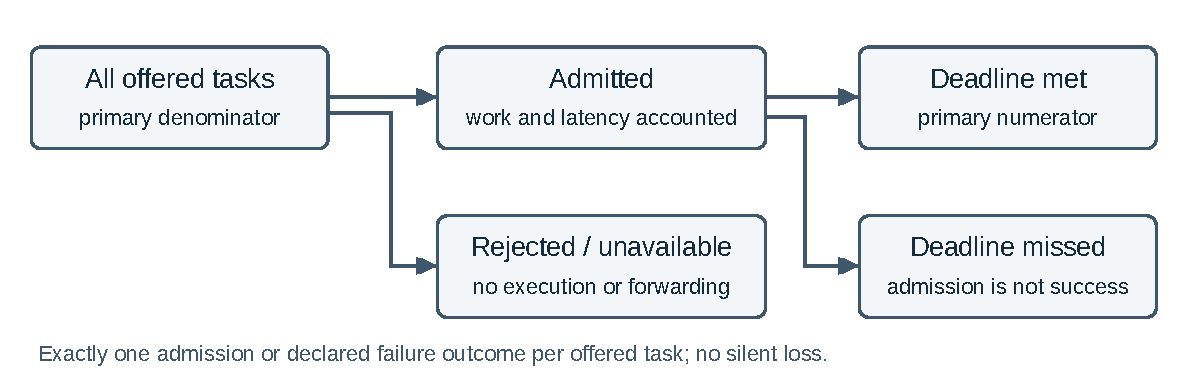
\includegraphics[width=\linewidth,height=.57\textheight,keepaspectratio]{assets/task_accounting.pdf}
\caption[Offered-task lifecycle]{Offered tasks remain in the primary denominator. Admission, execution assignment and deadline outcome are separate fields; selecting an RSU does not establish that work executed there. Reading: follow every offered task to an admission or terminal failure before interpreting deadline attainment.}\label{fig:3}
\end{figure}
% END SOURCE BLOCK 068

% BEGIN SOURCE BLOCK 069 paragraph
The inherited gate tests existing effective workload, including the candidate offset $O[i]$, against deadline $D[i]$:
% END SOURCE BLOCK 069

% BEGIN SOURCE BLOCK 070 equation
\begin{equation}\label{eq:3}
 W[r]+O[i]<D[i],\quad\text{together with an available task-count place.}
\end{equation}
% END SOURCE BLOCK 070

% BEGIN SOURCE BLOCK 071 paragraph
The inequality is strict. It excludes the candidate's service, radio transfer and forwarding cost, and therefore is a backlog filter rather than an end-to-end feasibility guarantee. Candidate ordering and offsets differ between algorithms (\S\,\ref{sec:2.5}). Admission uses positive ingress link quality as its coarse radio condition; the latency model additionally requires quality at least 0.15 for a usable transmission. Consequently, admission can still lead to a transmission-related deadline miss.
% END SOURCE BLOCK 071

% BEGIN SOURCE BLOCK 072 paragraph
For viable V2I execution, the modelled response latency is:
% END SOURCE BLOCK 072

% BEGIN SOURCE BLOCK 073 equation
\begin{equation}\label{eq:4}
 \begin{aligned}
 L_{\mathrm{raw}}[i]={}&T(\mathrm{input}[i],q,c)+W[r]+O[i]+s[i,r]\\
 &+T(0.001,q,c)+f\cdot\mathbf{1}(r\neq\mathrm{ingress}[i]).
 \end{aligned}
\end{equation}
% END SOURCE BLOCK 073

% BEGIN SOURCE BLOCK 074 paragraph
$T(b,q,c)$ is $0.1 + 1{,}000 \times 8b/c$ milliseconds for $q\geq 0.15$ and capacity $c>0.000000001$ Mbps, with $b$ in MB; otherwise it uses a $10^{9}$ ms failure value (up to the 0.1 ms propagation addition). The 0.001 MB return term reuses the ingress quality and capacity. It is not a separately simulated downlink or inter-RSU route. The fixed forwarding charge f is added once. Local latency is vehicle backlog plus local service; V2V adds input/return transfers on the selected peer link, peer backlog, preceding local/V2V reservations and peer service. Service $s$ derives from task cycles, device frequency, parallelism, utilisation and acceleration, with a sampled 0.9--1.1 multiplier. The placement code reserves the same sampled work used for latency: exact service knowledge is a declared information assumption.
% END SOURCE BLOCK 074

% BEGIN SOURCE BLOCK 075 paragraph
The gate-enabled paths pass final admission into latency scoring. Historical \path{off} instead passes earlier coarse eligibility while enqueueing uses refined admission: an in-substep capacity rejection need not receive penalty latency. Its historical numerical impact remains unquantified (\S\,\ref{sec:3.1}). The final mapping is $L[i]=10D[i]$ when $L_{\mathrm{raw}}[i]\geq 10^{8}$ ms, and $L[i]=L_{\mathrm{raw}}[i]$ otherwise. Finite late latencies are not generally clipped; success uses $L[i]\leq D[i]$, inclusively. Finite rejection latency alone is not a false deadline success.
% END SOURCE BLOCK 075

% BEGIN SOURCE BLOCK 076 paragraph
For each queue over an interval, work accounting requires:
% END SOURCE BLOCK 076

% BEGIN SOURCE BLOCK 077 equation
\begin{equation}\label{eq:5}
 W_{\mathrm{initial}}+\sum\text{admitted service}
 =\sum\text{served service}+W_{\mathrm{final}}.
\end{equation}
% END SOURCE BLOCK 077

% BEGIN SOURCE BLOCK 078 paragraph
This aggregate carry approximation has no individual departure-event model; Equation~\eqref{eq:5} checks its declared dynamics rather than physical calibration. After the fifth substep, $S[r]=\min(W_{\mathrm{post}}[r],1{,}000)$ is served and $W_{\mathrm{next}}[r]=W_{\mathrm{post}}[r]-S[r]$. If this empties the queue, its task count becomes zero. Otherwise the evaluator subtracts $\left\lfloor Q_{\mathrm{post}}[r]\times S[r]/W_{\mathrm{post}}[r]\right\rfloor$, retaining at least one task while positive work remains.
% END SOURCE BLOCK 078

\FloatBarrier
% BEGIN SOURCE BLOCK 079 heading
\subsection{Placement algorithms and their implementation}\label{sec:2.5}
% END SOURCE BLOCK 079

% BEGIN SOURCE BLOCK 080 paragraph
The inherited identifiers do not define canonical scheduling algorithms: \path{jsq} selects least service workload rather than shortest task count, and \path{dla} combines that common-target selector with Equation~\eqref{eq:3} \hyperref[source-s2]{[S2]}, \hyperref[source-s4]{[S4]}. The evaluator's own help text and source comment document that \path{jsq} and \path{dla} broadcast one argmin per substep to every V2I candidate, and that a randomised two-choice mode (\path{p2c}, \path{dla_p2c}) exists as a per-vehicle spreading alternative. Table~\ref{tab:3} makes their execution destination and gate switch explicit.
% END SOURCE BLOCK 080

% BEGIN SOURCE BLOCK 081 table
\begingroup
\singlespacing\footnotesize\setlength{\tabcolsep}{3pt}
\begin{xltabular}{\textwidth}{@{}YYYY@{}}
\caption[Infrastructure conditions]{Infrastructure conditions. All retain strongest-link radio ingress. ``Live'' eligibility is refreshed at each substep; the historical off mode retains step-entry coarse eligibility. \path{p2c} and \path{dla_p2c} are available; not evaluated. The other listed modes were evaluated. Reading: follow the fixed quantities and changed decision rules for each comparison.}\label{tab:3} \\
\toprule
Mode & Execution destination & Backlog gate & Coarse eligibility \\
\midrule\endfirsthead
\toprule
Mode & Execution destination & Backlog gate & Coarse eligibility \\
\midrule\endhead
\bottomrule\endfoot
\path{off} & Ingress & Off & Step entry \\
\path{jsq} & Common least-workload target & Off & Live \\
\path{ingress_dla} & Ingress & On & Live \\
\path{dla} & Common least-workload target & On & Live \\
\path{per_task_dla} & Causal least-workload target & On & Live \\
\path{causal_round_robin} & Persistent cyclic target & On & Live \\
\path{p2c} & Per-vehicle two random candidates, least workload & Off & Live \\
\path{dla_p2c} & Per-vehicle two random candidates, least workload & On & Live \\
\end{xltabular}
\endgroup
% END SOURCE BLOCK 081

% BEGIN SOURCE BLOCK 082 paragraph
Both placement algorithms below operate once per task substep, using its entry state $W$, Q. Index $i$ follows ascending padded-vehicle order, not arrival-time or deadline priority. Each candidate has actual service $s[i,r]$, deadline $D[i]$ and a fixed actor action and radio ingress. Every argmin considers all RSUs and breaks ties by lowest index; a full selected RSU is rejected rather than excluded and retried elsewhere.
% END SOURCE BLOCK 082

% BEGIN SOURCE BLOCK 083 paragraph
Proposition~\ref{prop:1} supplies an exact-model guarantee under stated assumptions, not a blanket float32 guarantee. For common-target reconciliation, let $E[i]$ mean active V2I attempt, positive ingress quality and $Q[r[i]]<C$ at substep entry. For an admission mask $M$, define $O[i,M]$ as the sum of $s[j,r[i]]$ over earlier $j<i$ with the same target and $M[j]$ true; $H[i,M]$ is their count. Offsets are exclusive: a candidate's own service is omitted. Algorithm~\ref{alg:1} performs exactly three simultaneous replacements.
% END SOURCE BLOCK 083

% BEGIN SOURCE BLOCK 084 algorithm
\begin{algorithm}[htbp]
\caption{common-target placement with gate (one substep)}\label{alg:1}
\begin{Verbatim}[fontsize=\small,breaklines=true]
r[i] = lowest-index argmin(W), shared by all candidates
M = E
repeat exactly three times:
    compute O[i,M] and H[i,M] from the previous whole mask
    M_new[i] = E[i] and (W[r[i]] + O[i,M] < D[i])
                       and (H[i,M] < C - Q[r[i]])
    M = M_new simultaneously
recompute final offsets O[i,M] for latency
label E-candidates failing the final workload test as gate failures
label remaining E-candidates excluded by M as capacity failures
commit each M-admitted task and its full service once
unavailable or rejected tasks reserve nothing
\end{Verbatim}
\end{algorithm}
% END SOURCE BLOCK 084

% BEGIN SOURCE BLOCK 085 paragraph
Target selection never changes during reconciliation. The retained mask and recomputed offsets determine recorded processing. Section~\ref{sec:3.5} distinguishes the exact guarantee from its float32 boundary. Ingress with the gate uses the same offset/reconciliation machinery with individual ingress targets instead of the common argmin. Gate-off modes omit the workload test.
% END SOURCE BLOCK 085

% BEGIN SOURCE BLOCK 086 algorithm
\begin{algorithm}[htbp]
\caption{causal per-task placement with gate (one substep)}\label{alg:2}
\begin{Verbatim}[fontsize=\small,breaklines=true]
repeat exactly three complete passes:
    working_W = W; working_Q = Q       # restart, not cumulative
    for i in ascending padded-vehicle order:
        r[i] = lowest-index argmin(working_W)
        O[i] = working_W[r[i]] - W[r[i]]
        require active V2I, positive quality and Q[r[i]] < C
        test working_W[r[i]] < D[i], then working_Q[r[i]] < C
        if admitted:
            working_W[r[i]] += s[i,r[i]]
            working_Q[r[i]] += 1
        otherwise label failure; reserve nothing
retain the last pass; commit its admitted work once
\end{Verbatim}
\end{algorithm}
% END SOURCE BLOCK 086

% BEGIN SOURCE BLOCK 087 paragraph
This intervention changes selection frequency, reservation visibility and reconciliation semantics, rather than argmin frequency alone. Repeated passes restart identically and commit once; they neither triple reservations nor drain service between substeps. The causal gate and capacity see earlier admissions immediately.
% END SOURCE BLOCK 087

% BEGIN SOURCE BLOCK 088 paragraph
Figure~\ref{fig:4} is a constructed mechanics example, neither a recorded task group nor an estimate of recoverable historical failures. Assume three empty identical RSUs, four viable 40 ms tasks with 100 ms deadlines, nonbinding capacity and negligible communication. Common-target chooses RSU 0; its masks settle at three admissions and one gate rejection. The admitted offsets are 0, 40 and 80 ms, leaving 120, 0, 0 ms: the third admitted task misses its deadline despite passing the backlog gate. Per-task selects 0, 1, 2, 0, leaves 80, 40, 40 ms and all four meet deadlines under these assumptions.
% END SOURCE BLOCK 088

% BEGIN SOURCE BLOCK 089 figure
\begin{figure}[htbp]
\centering
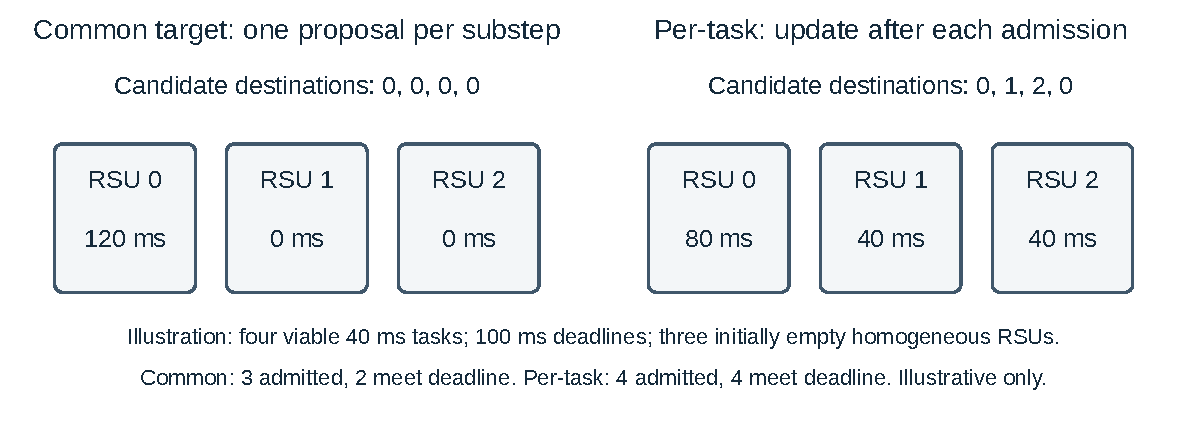
\includegraphics[width=\linewidth,height=.57\textheight,keepaspectratio]{assets/dispatch_example.pdf}
\caption[Illustrative dispatch comparison]{Four illustrative proposals. The common destination remains fixed through reconciliation; causal placement updates after admissions. The accompanying worked example states admissions and deadline outcomes under deliberately simplified assumptions. Reading: compare the unchanged common destination with immediate reservations and reselection after each admitted task.}\label{fig:4}
\end{figure}
% END SOURCE BLOCK 089

\FloatBarrier
% BEGIN SOURCE BLOCK 090 heading
\subsection{Experimental progression and inference}\label{sec:2.6}
% END SOURCE BLOCK 090

% BEGIN SOURCE BLOCK 091 paragraph
E0 and E1 form the validation and scoping stage. E0 supplies the recorded measurement foundation; E1 compares three queue limits at fixed service over five matched draws; E2/E2b explore placement and admission on one draw. E2c compares common-target with ingress on new incident seeds 1--4. After inspecting them, E2d adds per-task placement on those same draws and reuses their controls: an adaptive extension, not new independent observations \hyperref[source-s0]{[S0]}--\hyperref[source-s3]{[S3]}.
% END SOURCE BLOCK 091

% BEGIN SOURCE BLOCK 092 paragraph
The morning pilot uses seed 1 for ingress and per-task placement. After inspecting it, the replication declares seeds 0, 2, 3 and 4 and all three arms, yielding twelve new full runs. The primary contrasts are per-task minus ingress, common-target minus ingress, and per-task minus common-target. The pilot is excluded; a supplementary two-arm five-draw summary is descriptive. The local protocol and manifest preceded the new outcomes, but there was no external preregistration \hyperref[source-s7]{[S7]}, \hyperref[source-s8]{[S8]}.
% END SOURCE BLOCK 092

% BEGIN SOURCE BLOCK 093 paragraph
For each contrast, a fleet draw supplies one paired difference in percentage points. Draws receive equal weight. The mean difference has a Student-$t$ interval, $\text{mean}\pm t\times\frac{\text{sample standard deviation}}{\sqrt{n}}$. Incident E2c/E2d retain their reported individual 95\% intervals. The original morning protocol additionally uses Bonferroni simultaneous intervals for three contrasts, with critical value $t$ at probability $1-0.05/(2\times 3)$, three degrees of freedom. Its reversal criterion requires the simultaneous common-target-minus-ingress interval below zero and the per-task-minus-ingress interval above zero. Four draws cannot strongly diagnose distributional assumptions; these small-sample intervals remain conditional parametric summaries, not task-level significance tests.
% END SOURCE BLOCK 093

% BEGIN SOURCE BLOCK 094 paragraph
The later confirmation uses eight paired fleet/evaluator-seed blocks, (100,200) through (107,207), and four arms: ingress, common-target, per-task and causal round-robin. Controls, rotating arm order and analysis were sealed before full outcomes. Per-task minus ingress, common-target minus ingress and per-task minus round-robin receive equal block weights and two-sided Bonferroni simultaneous 95\% Student-$t$ intervals, df=7. The same two-direction criterion tests recurrence; original draws and pilots remain separate. Independent joint blocks and approximately normal paired effects remain assumptions that eight blocks cannot strongly diagnose \hyperref[source-s16]{[S16]}.
% END SOURCE BLOCK 094

\FloatBarrier
% BEGIN SOURCE BLOCK 095 heading
\subsection{Sensitivities, mechanism audit and validation}\label{sec:2.7}
% END SOURCE BLOCK 095

% BEGIN SOURCE BLOCK 096 paragraph
The state-information pilot uses incident seed 1 and report ages 0, 100, 500 and 1,000 ms, alongside ingress. The report ages follow Dr Sampaio's suggestion of 100 ms, 500 ms and 1 s. Admission remains live. For previous post-admission workload B and positive age $d$, the report is $\max(B-(1{,}000-d),0)$, with current-batch reservations added immediately. This assumes continuous service between batches without redistributing arrivals. Startup uses live state and recorded age zero \hyperref[source-s5]{[S5]}.
% END SOURCE BLOCK 096

% BEGIN SOURCE BLOCK 097 paragraph
Four ten-step forwarding probes qualify fixed-latency transformations of saved full records: charges leave admission, queues and actions unchanged. No full positive-cost simulation or network model is implied; penalty-equal ambiguity remains unresolved \hyperref[source-s6]{[S6]}.
% END SOURCE BLOCK 097

% BEGIN SOURCE BLOCK 098 paragraph
Execution fields record admitted assignment, not departures \hyperref[source-s13]{[S13]}. Morning checks covered matched inputs/actions and full/probe prefixes, with logit tolerance 0.00001 and workload-balance error up to about 0.00174 ms \hyperref[source-s8]{[S8]}. The September audit independently identifies offers from active masks, V2I admission from enqueue fields and non-V2I failures from rejection predicates, then reconciles flags, categories, latency/deadlines, assignments and summaries.
% END SOURCE BLOCK 098

% BEGIN SOURCE BLOCK 099 paragraph
Task joins require matched trace-row/substep/slot coordinates and corresponding fleet, task, arrival, action and ingress fields. Unsaved sizes correspond through the arm-independent key schedule. Gains minus losses must equal the success difference over the common offered denominator; later queues can diverge, so these are descriptive transitions.
% END SOURCE BLOCK 099

% BEGIN SOURCE BLOCK 100 paragraph
Retrospective diagnostics distinguish simultaneous common-target admission A, causal admission replaying A's targets B, and causal reselection C. The completed proof and numerical investigation are retained in Appendix~\ref{app:C}, separately from observed fleet results \hyperref[source-s14]{[S14]}.
% END SOURCE BLOCK 100

\FloatBarrier
% BEGIN SOURCE BLOCK 101 heading
\subsection{Cyclic comparator and retrospective measurement design}\label{sec:2.8}
% END SOURCE BLOCK 101

% BEGIN SOURCE BLOCK 102 paragraph
Causal round-robin isolates workload awareness from spreading. Its pointer starts at RSU 0, persists across substeps/batches, and advances modulo $R$ for every active positive-radio V2I attempt, including rejections. Unavailable radio and padding do not advance it; there is no retry or full-node skipping. Order, sampled work, gate/capacity, precision, accounting, forwarding and drain match per-task placement. Repeated passes restart identically; the pointer commits once. A versioned evaluator preserves frozen implementations. Qualification checks compatibility, shared inputs, admission accounting and restart; Appendix~\ref{app:E} bounds coverage \hyperref[source-s15]{[S15]}, \hyperref[source-s16]{[S16]}.
% END SOURCE BLOCK 102

% BEGIN SOURCE BLOCK 103 paragraph
Scheduler timing uses actual JAX helpers, including three-replacement prefixes; precomputed candidate work replaces only the service provider. Sixteen configurations combine four arms, $N/R=215/9$ or 2,488/10, $K=5$ and sparse/empty or busy/nonempty fixtures. Arms share arrays with coupled type/deadline/service values. Busy entry queues are imposed stress states, excluded by exact clearing from empty initialisation (\S\,\ref{sec:3.5}). Following JAX guidance, compilation is separate, inputs are device-resident, five warm-ups precede 100 synchronised calls. Actor, radio, service generation, transfer, scoring and I/O are excluded. Repetitions measure host variability, not fleet uncertainty \cite{ref14}.
% END SOURCE BLOCK 103

% BEGIN SOURCE BLOCK 104 paragraph
Retrospective type aggregation retains all types and draws without subgroup significance tests, using the eight authenticated ingress/per-task files from the original four-draw morning sample. Categories supply admission, gate rejection and admitted misses; type totals must reproduce all-task summaries and paired net changes.
% END SOURCE BLOCK 104

\FloatBarrier
% BEGIN SOURCE BLOCK 105 heading
\section{Evaluation and Reflection}\label{sec:3}
% END SOURCE BLOCK 105

\FloatBarrier
% BEGIN SOURCE BLOCK 106 heading
\subsection{Validation and scoping: accounting and historical capacity}\label{sec:3.1}
% END SOURCE BLOCK 106

% BEGIN SOURCE BLOCK 107 paragraph
E0 addressed a concrete mismatch between task scoring and queue admission. In the legacy clamp path, the evaluator scored eligible V2I tasks and multiplied their combined service work by the fraction fitting the task-count ceiling. Surplus tasks were not individually identified in earlier scoring. The 5 August repair introduced per-task admission/rejection and full enqueueing of admitted work. Putra implemented the repair after I identified the mismatch between task scoring and queue admission; E0 qualified recorded accounting in that configuration \hyperref[source-s0]{[S0]}, \hyperref[source-s12]{[S12]}.
% END SOURCE BLOCK 107

% BEGIN SOURCE BLOCK 108 paragraph
Consider a constructed explanation, not an observed historical pair: one queue place remains and two viable tasks each require 40 ms. Legacy fractional enqueue adds (1/2) \ensuremath{\times} 80 = 40 ms, although both can remain in the scored population. With unequal services, fractional enqueue can also differ from the work of the particular admitted task. Reject-mode admission instead accepts one task in order, enqueues its full 40 ms and assigns the other a failure.
% END SOURCE BLOCK 108

% BEGIN SOURCE BLOCK 109 paragraph
The relevant invariant is that offers partition into admissions and terminal failures, with no execution or success assigned to rejected work. E0's negative fixture changes the summary offered count without adding a task record and must fail. Summary work partition alone is weaker: rejected work is calculated as offered minus admitted. Later reconstruction instead checks enqueue, drain and queue endpoints independently.
% END SOURCE BLOCK 109

% BEGIN SOURCE BLOCK 110 paragraph
Archived E0 receipts report passing their checks, but source inspection identifies a remaining exception in E0/E1 and E2's reused off path: coarse eligibility reaches latency scoring while refined admission governs enqueueing. Recorded capacity rejections establish exposure, not false successes. Raw per-task arrays for E0, E1 and E2 were not retained; their run summaries, validation receipts and manifests are archived and reproduce the reported intervals. The task-level impact of the scoring-mask exception therefore cannot be quantified for those studies; Appendix~\ref{app:B} distinguishes this gap from later audit coverage \hyperref[source-s13]{[S13]}.
% END SOURCE BLOCK 110

% BEGIN SOURCE BLOCK 111 paragraph
E1 varied waiting-room capacity across five matched draws. The archived score difference for 99,520 versus 1,866 tasks per RSU was \ensuremath{-}0.01094 percentage points, with a 95\% interval [\ensuremath{-}0.02465, +0.00276]. Recalculation from surviving run summaries reproduces this interval; it is not fresh task-level validation. The archived E1 score contrast is statistically inconclusive under the historical implementation. Its interpretation as admission-consistent deadline attainment remains qualified by the unquantified scoring-mask exception. The interval describes sampling uncertainty conditional on that implementation, not the additional measurement uncertainty. Neither equivalence nor statistically supported degradation follows \hyperref[source-s1]{[S1]}.
% END SOURCE BLOCK 111

% BEGIN SOURCE BLOCK 112 paragraph
The saved secondary summaries report more admissions and lower rejection at larger limits, while mean admitted latency rises from approximately 3.77 to 12.19 and 132.49 seconds. These changing admitted populations cannot substitute for the offered-task contrast; their latency summaries retain the scoring-mask qualification. More retained work need not mean more useful service.
% END SOURCE BLOCK 112

% BEGIN SOURCE BLOCK 113 paragraph
Changing the off scoring mask could affect transmit energy, SoC and later observations: even admission-consistent saved flags would describe fixed history, not a corrected rerun. Separately, the completed audit found no non-admitted successes or non-penalty rejection latencies in 19 authenticated September gate-enabled runs, with admission/category/summary agreement. It supports those outcomes without resolving historical measurement impact.
% END SOURCE BLOCK 113

\FloatBarrier
% BEGIN SOURCE BLOCK 114 heading
\subsection{From admission decomposition to the incident reversal}\label{sec:3.2}
% END SOURCE BLOCK 114

% BEGIN SOURCE BLOCK 115 paragraph
E2's exploratory seed-0 comparison showed offered attainment of approximately 68.362\% for strongest-link execution without the deadline gate, 67.568\% for inherited least-busy placement without the gate, and 69.494\% for inherited least-busy placement with the gate. The last comparison changed both placement and admission relative to the strongest-link reference. Its improvement could not establish that load balancing itself helped \hyperref[source-s2]{[S2]}.
% END SOURCE BLOCK 115

% BEGIN SOURCE BLOCK 116 paragraph
E2b added ingress execution with the same deadline gate, reaching approximately 71.577\%. The strongest-link contrast was +3.215 points and the common-target contrast +1.926 points, giving an interaction of \ensuremath{-}1.290 points. However, \path{off} uses step-entry coarse saturation eligibility while \path{ingress_dla} refreshes eligibility per substep. Their contrast and interaction bundle the gate with this timing difference and retain the legacy scoring-mask exception (\S\,\ref{sec:2.4}). The manifest records 138 unavailable V2I attempts among 13,076,234 offered tasks in off; that count does not bound downstream effects. E2b identifies a stronger comparator without assigning its entire gain solely to the gate. Subsequent gate-held placement comparisons use live eligibility and refined scoring masks in all arms. In the exploratory draw, common-target remained 2.083 points below ingress with the gate.
% END SOURCE BLOCK 116

% BEGIN SOURCE BLOCK 117 paragraph
E2c tested the common-target comparison on four new incident fleet draws, excluding discovery seed 0. Its mean difference from ingress was \ensuremath{-}2.122 points, with an individual 95\% interval of [\ensuremath{-}2.234, \ensuremath{-}2.011]. All four paired differences were negative. The inherited scheduler selects one least-workload target per task substep and assigns it to every V2I candidate in that substep, a behaviour recorded in the evaluator's documentation. I chose to test a causal per-task implementation rather than the evaluator's randomised two-choice mode, because it isolates target timing and reservation visibility while holding the least-workload criterion fixed; the two-choice mode remains the first comparator to add (Section~\ref{sec:4.3}). E2d introduced the causal per-task implementation under the same actor, trace, gate predicate, queue ceiling, service and forwarding controls. Table~\ref{tab:4} retains all four draw-level results \hyperref[source-s3]{[S3]}.
% END SOURCE BLOCK 117

% BEGIN SOURCE BLOCK 118 table
\Needspace{14\baselineskip}
\begingroup
\singlespacing\footnotesize\setlength{\tabcolsep}{3pt}
\begin{xltabular}{\textwidth}{@{}YYYYY@{}}
\caption[Incident attainment]{Incident offered-task deadline attainment, expressed as percentages. E2d reused the exact E2c ingress and common-target controls; these are four paired draws, not separate sets of independent controls. Reading: compare policies within the same incident fleet draw.}\label{tab:4} \\
\toprule
Fleet seed & Ingress & Common-target & Per-task & Per-task \ensuremath{-} ingress, pp \\
\midrule\endfirsthead
\toprule
Fleet seed & Ingress & Common-target & Per-task & Per-task \ensuremath{-} ingress, pp \\
\midrule\endhead
\bottomrule\endfoot
1 & 72.003 & 69.794 & 72.467 & +0.464 \\
2 & 70.369 & 68.317 & 70.956 & +0.587 \\
3 & 70.298 & 68.153 & 70.805 & +0.507 \\
4 & 70.887 & 68.805 & 71.438 & +0.551 \\
\end{xltabular}
\endgroup
% END SOURCE BLOCK 118

% BEGIN SOURCE BLOCK 119 paragraph
Per-task exceeds ingress by 0.527 points, individual 95\% interval [+0.442, +0.612], and common-target by 2.649 points, interval [+2.621, +2.678]. RQ1 therefore yields opposite rankings for the two implementations. These intervals summarise an adaptive extension on examined draws; the morning protocol supplies prospective replication.
% END SOURCE BLOCK 119

% BEGIN SOURCE BLOCK 120 paragraph
Neither arm establishes optimal dispatch; the conversions here describe the observed mean. The larger +2.649-point common-target contrast diagnoses that implementation rather than the gain over the stronger reference. Against ingress attainment of 70.889\%, the +0.527-point difference means about 53 extra successes per 10,000 offered, or a 0.744\% relative increase.
% END SOURCE BLOCK 120

\FloatBarrier
% BEGIN SOURCE BLOCK 121 heading
\subsection{Morning replication with the inspected pilot excluded}\label{sec:3.3}
% END SOURCE BLOCK 121

% BEGIN SOURCE BLOCK 122 paragraph
The inspected morning pilot offered 1,744,116 tasks and produced 91.075\% ingress versus 94.028\% per-task attainment: +2.953 points or 51,503 successes. It motivated replication but remains exploratory \hyperref[source-s7]{[S7]}.
% END SOURCE BLOCK 122

% BEGIN SOURCE BLOCK 123 paragraph
The morning protocol declared four new seeds and all three arms before outcomes. Table~\ref{tab:5} reproduces common-target < ingress < per-task in every draw. Mean attainment is 85.655\%, 88.887\% and 92.785\%, respectively; its lower ingress/per-task means than the pilot underline the need for replication \hyperref[source-s8]{[S8]}.
% END SOURCE BLOCK 123

% BEGIN SOURCE BLOCK 124 table
\begingroup
\singlespacing\footnotesize\setlength{\tabcolsep}{3pt}
\begin{xltabular}{\textwidth}{@{}YYYYY@{}}
\caption[Morning primary replication]{Morning primary replication. Seed 1 is absent because it was the inspected pilot; each row is a matched fleet draw on the same morning trace. Reading: compare policies within a row; the inspected pilot is absent.}\label{tab:5} \\
\toprule
Fleet seed & Ingress, \% & Common-target, \% & Per-task, \% & Per-task \ensuremath{-} ingress, pp \\
\midrule\endfirsthead
\toprule
Fleet seed & Ingress, \% & Common-target, \% & Per-task, \% & Per-task \ensuremath{-} ingress, pp \\
\midrule\endhead
\bottomrule\endfoot
0 & 88.817 & 85.660 & 92.705 & +3.888 \\
2 & 87.536 & 83.537 & 92.060 & +4.524 \\
3 & 89.082 & 85.862 & 92.978 & +3.896 \\
4 & 90.113 & 87.559 & 93.399 & +3.286 \\
\end{xltabular}
\endgroup
% END SOURCE BLOCK 124

% BEGIN SOURCE BLOCK 125 paragraph
Table~\ref{tab:6}'s simultaneous per-task-minus-ingress interval is positive and common-target-minus-ingress interval negative, satisfying the prespecified reversal criterion. Figure~\ref{fig:5} displays these primary results.
% END SOURCE BLOCK 125

% BEGIN SOURCE BLOCK 126 table
\begingroup
\singlespacing\footnotesize\setlength{\tabcolsep}{3pt}
\begin{xltabular}{\textwidth}{@{}YYYY@{}}
\caption[Morning paired contrasts]{Morning paired contrasts in percentage points. Individual intervals are two-sided 95\% Student-$t$ intervals; simultaneous intervals use the prespecified three-contrast Bonferroni adjustment. Replication uses four fleet draws. Reading: use the simultaneous intervals for the declared three-contrast decision.}\label{tab:6} \\
\toprule
Contrast & Mean & Individual 95\% interval & Simultaneous 95\% interval \\
\midrule\endfirsthead
\toprule
Contrast & Mean & Individual 95\% interval & Simultaneous 95\% interval \\
\midrule\endhead
\bottomrule\endfoot
Per-task \ensuremath{-} ingress & +3.899 & [+3.094, +4.703] & [+2.671, +5.126] \\
Common-target \ensuremath{-} ingress & \ensuremath{-}3.232 & [\ensuremath{-}4.176, \ensuremath{-}2.289] & [\ensuremath{-}4.672, \ensuremath{-}1.793] \\
Per-task \ensuremath{-} common-target & +7.131 & [+5.385, +8.877] & [+4.466, +9.795] \\
\end{xltabular}
\endgroup
% END SOURCE BLOCK 126

% BEGIN SOURCE BLOCK 127 figure
\begin{figure}[htbp]
\centering
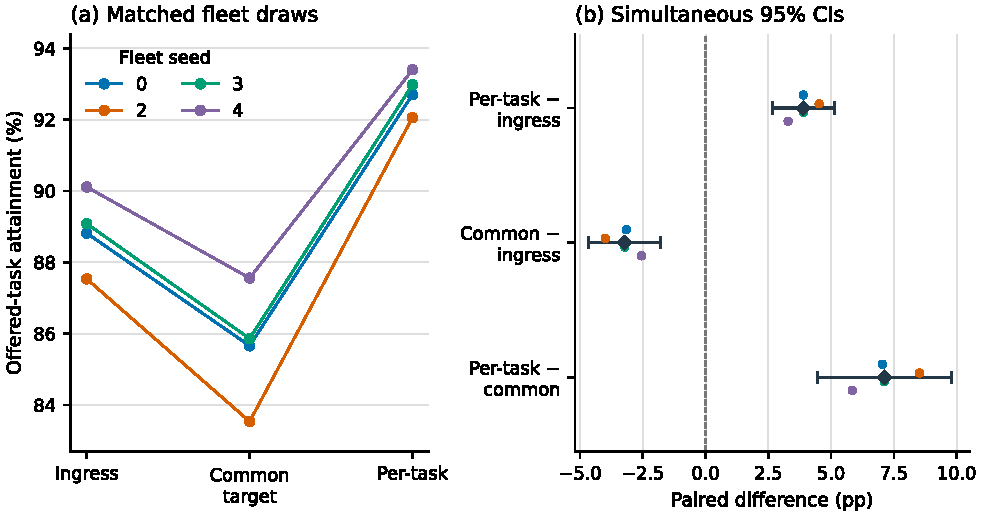
\includegraphics[width=\linewidth,height=.57\textheight,keepaspectratio]{assets/primary_replication.pdf}
\caption[Four-draw morning replication]{Redrawn from archived morning primary data. Left: within-draw attainment. Right: draw differences, mean diamonds and three-contrast Bonferroni intervals. The inspected pilot is excluded; uncertainty concerns four newly declared fleet draws, conditional on the frozen actor and morning scenario \hyperref[source-s8]{[S8]}. Reading: read the four new fleet draws as matched replications and the adjusted intervals as the declared contrast family.}\label{fig:5}
\end{figure}
% END SOURCE BLOCK 127

% BEGIN SOURCE BLOCK 128 paragraph
The five-draw ingress/per-task mean including the pilot is +3.709 points descriptively, outside Table~\ref{tab:6}; no common-target pilot result is available.
% END SOURCE BLOCK 128

% BEGIN SOURCE BLOCK 129 paragraph
The larger morning effect cannot be attributed solely to density: RSU layout/count, date, duration, padded fleet width and entry conventions also change. Separate scenario analyses support recurrence rather than a pooled geographical effect. The morning gain is about 390 extra successes per 10,000 offered, a 4.386\% relative increase over ingress.
% END SOURCE BLOCK 129

\FloatBarrier
% BEGIN SOURCE BLOCK 130 heading
\subsection{Confirmation under joint randomness and comparison with cyclic spreading}\label{sec:3.4}
% END SOURCE BLOCK 130

% BEGIN SOURCE BLOCK 131 paragraph
All 32 full morning cells and eight block-control receipts passed after bounded qualification, with no failed attempts, retries or exclusions. Table~\ref{tab:7} reports the declared contrasts; Appendix~\ref{app:E} retains every block \hyperref[source-s16]{[S16]}.
% END SOURCE BLOCK 131

% BEGIN SOURCE BLOCK 132 paragraph
Evaluator seed varies observation descriptors, arrivals, operational types/sizes, fading and service wobble; fleet seed varies tier, EV status and initial SoC. The estimand remains the total scheduling intervention under frozen weights, without forcing replay or guaranteeing future action equality. Small observation and logit differences occurred in block 1; they did not change actions. All four arms shared the required exogenous arrays exactly within each block, and actions matched exactly in all 24 non-reference arm/block comparisons.
% END SOURCE BLOCK 132

% BEGIN SOURCE BLOCK 133 table
\begingroup
\singlespacing\footnotesize\setlength{\tabcolsep}{3pt}
\begin{xltabular}{\textwidth}{@{}YYY@{}}
\caption[Eight-block simultaneous contrasts]{New morning confirmation, eight paired joint-seed blocks with equal weighting. Two-sided Bonferroni simultaneous 95\% Student-$t$ intervals cover the three predeclared contrasts; positive differences favour the first arm. Reading: both reversal directions and the cyclic-control increment are assessed in one three-contrast family.}\label{tab:7} \\
\toprule
Contrast & Mean difference, pp & Simultaneous 95\% interval, pp \\
\midrule\endfirsthead
\toprule
Contrast & Mean difference, pp & Simultaneous 95\% interval, pp \\
\midrule\endhead
\bottomrule\endfoot
Per-task \ensuremath{-} ingress & +4.137 & [+3.556, +4.717] \\
Common-target \ensuremath{-} ingress & \ensuremath{-}3.504 & [\ensuremath{-}3.980, \ensuremath{-}3.028] \\
Per-task \ensuremath{-} round-robin & +0.631 & [+0.511, +0.750] \\
\end{xltabular}
\endgroup
% END SOURCE BLOCK 133

% BEGIN SOURCE BLOCK 134 paragraph
The declared reversal criterion holds, evaluated using both directional requirements within the same simultaneous family. The mean per-task difference corresponds to +413.7 successes per 10,000 offered tasks relative to ingress. Workload-aware targeting outperformed cyclic spreading in this study. Its mean benefit is 63.1 successes per 10,000 offered tasks over round-robin, accompanying higher scheduler-only cost on the separate fixtures in Table~\ref{tab:8}.
% END SOURCE BLOCK 134

% BEGIN SOURCE BLOCK 135 paragraph
Figure~\ref{fig:6} shows all four arms in each of the eight blocks, rather than reusing the earlier four-draw plot for this confirmation. Equal block weighting gives mean attainment of 88.372\% for ingress, 91.879\% for round-robin and 92.509\% for per-task placement. The descriptive round-robin-minus-ingress difference is +3.506 percentage points, and the further per-task-minus-round-robin increment is +0.631 points. Their sum is the +4.137-point per-task-minus-ingress difference \hyperref[source-s16]{[S16]}.
% END SOURCE BLOCK 135

% BEGIN SOURCE BLOCK 136 paragraph
The unrounded mean increments give \textbf{84.8\% for ingress-to-round-robin and 15.2\% for the additional round-robin-to-per-task step}. These are descriptive shares of arm-mean differences, not causal mechanism shares or a fourth declared inferential contrast. The closer workload-awareness comparison is per-task versus causal round-robin: cyclic spreading captures most of the ingress gain, with a smaller, consistently positive workload-aware increment.
% END SOURCE BLOCK 136

% BEGIN SOURCE BLOCK 137 figure
\begin{figure}[htbp]
\centering
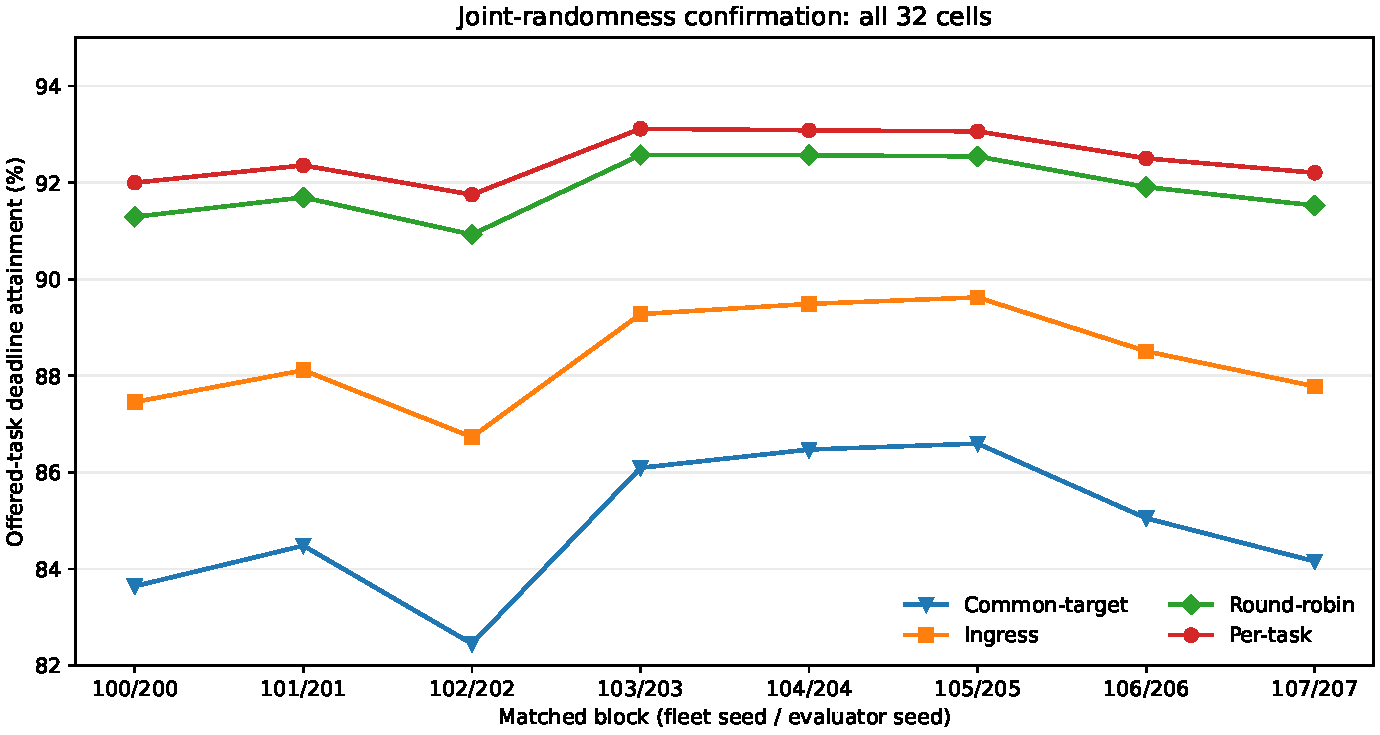
\includegraphics[width=\linewidth,height=.57\textheight,keepaspectratio]{assets/joint_confirmation_eight_blocks.pdf}
\caption[All eight joint-randomness blocks]{Offered-task deadline attainment recomputed as 100 times successes divided by offers for each of the 32 archived cells. Lines connect the same policy across eight matched blocks; block labels show fleet/evaluator seeds. No tasks are treated as independent replications and no uncertainty intervals are inferred from the line segments \hyperref[source-s16]{[S16]}. Reading: every block retains common-target below ingress and per-task above round-robin; Table~\ref{tab:7} supplies the declared simultaneous intervals.}\label{fig:6}
\end{figure}
% END SOURCE BLOCK 137

% BEGIN SOURCE BLOCK 138 paragraph
The critical value is 3.127552 with seven degrees of freedom; full controls are in Appendix~\ref{app:E}. Joint randomness does not vary geography, actor training or the physical model. It extends the original fleet-conditional finding to new evaluator streams.
% END SOURCE BLOCK 138

\FloatBarrier
\clearpage
% BEGIN SOURCE BLOCK 139 heading
\subsection{Why destination semantics matter}\label{sec:3.5}
% END SOURCE BLOCK 139

% BEGIN SOURCE BLOCK 140 paragraph
Common-target placement assigned morning work only to RSUs 0--4, whereas causal per-task placement used all nine. With $K$ substeps and $R$ RSUs, selecting one destination per substep admits new work to at most $\min(K,R)$ destinations in a batch. Empty starts, lowest-index ties, positive admissions and no intervening drain further produce the recurring low-index prefix. Under the exact gate/service model, workload remains below 538.889 ms before the 1,000 ms drain, explaining the recurring empty starts. Appendix~\ref{app:C} retains the reconstructed states and Figure~\ref{fig:8} \hyperref[source-s8]{[S8]}, \hyperref[source-s9]{[S9]}.
% END SOURCE BLOCK 140

% BEGIN SOURCE BLOCK 141 proposition
\begin{proposition}[fixed-target admission in the studied exact model]\label{prop:1}
Fix candidate order, eligibility, destinations, initial nonnegative workload/count and nonnegative service demands, with strict backlog and exclusive count-capacity tests and no intervening drain. At each nonempty destination, let $n$ be the eligible candidate count and $d$ the number of distinct deadlines. Starting from the eligibility mask, simultaneous replacement reaches the unique causal fixed point within $\min(n,2d-1)$ replacements; destinations decouple.\end{proposition}
% END SOURCE BLOCK 141

% BEGIN SOURCE BLOCK 142 paragraph
With the studied two deadline values, the bound is three replacements in exact arithmetic. This rules out unrestricted fixed-target reconciliation failure as an explanation within that model; it does not equate fixed targets with reselection or exact arithmetic with float32 execution. The proof, numerical boundaries and adverse example are retained together in Appendix~\ref{app:C} \hyperref[source-s14]{[S14]}.
% END SOURCE BLOCK 142

% BEGIN SOURCE BLOCK 143 paragraph
Matched outcome accounting in the original four-draw morning sample records 284,821 gained successes and 12,842 losses, for 271,979 net successes. Gate-rejection recovery supplies most gains. These are descriptive transitions under diverging later queues, not individual-decision causal effects. Tables C2 and C3 preserve the full transitions and type breakdown in Appendix~\ref{app:C}: the mechanism concentrates destinations, while the outcome accounting shows where attainment changes.
% END SOURCE BLOCK 143

\FloatBarrier
\clearpage
% BEGIN SOURCE BLOCK 144 heading
\subsection{Bounded state-information and forwarding sensitivities}\label{sec:3.6}
% END SOURCE BLOCK 144

% BEGIN SOURCE BLOCK 145 paragraph
In incident seed 1, fresh per-task attainment was 72.46695\%, versus ingress 72.00328\%. Report ages 100, 500 and 1,000 ms yielded 72.46695\%, 72.46856\% and 72.45510\%; single-draw changes do not establish equivalence or population robustness \hyperref[source-s5]{[S5]}.
% END SOURCE BLOCK 145

% BEGIN SOURCE BLOCK 146 paragraph
Every 100 ms report equalled fresh state over 35,990 non-startup RSU/batch observations: queues had emptied, making that treatment inactive. Reports differed at 500 ms in 79.58\% of observations and at 1,000 ms in all. Live admission and immediate reservations protect this older-report model; stale capacity, delayed acknowledgements or dispersed arrivals would change it. Equal outcomes do not establish harmless communication delay.
% END SOURCE BLOCK 146

% BEGIN SOURCE BLOCK 147 paragraph
Fixed forwarding overheads 0, 1, 2.5, 5 and 10 ms yielded 72.46695\%, 72.44783\%, 72.41882\%, 72.37240\% and 72.28579\% attainment. At 10 ms the advantage remained 0.28251 points, or 36,942 successes over ingress, despite 23,689 extra misses relative to zero overhead \hyperref[source-s6]{[S6]}.
% END SOURCE BLOCK 147

% BEGIN SOURCE BLOCK 148 paragraph
These are saved-record transformations qualified by four short direct probes. Forwarding charges do not feed back into admission, queues or actions in that path; the calculation models neither congestion nor postponed arrivals. A further 104 forwarded tasks had penalty-equal latency ambiguity but were already misses and remained misses under every nonnegative charge. Their latency ambiguity remains unresolved. RQ3 supports the tested information and fixed-cost models, not an extrapolated break-even threshold or network design.
% END SOURCE BLOCK 148

\FloatBarrier
% BEGIN SOURCE BLOCK 149 heading
\subsection{Computational trade-offs and research implementation}\label{sec:3.7}
% END SOURCE BLOCK 149

% BEGIN SOURCE BLOCK 150 table
\begingroup
\singlespacing\footnotesize\setlength{\tabcolsep}{3pt}
\begin{xltabular}{\textwidth}{@{}YYYYY@{}}
\caption[Scheduler-only engineering trade-offs]{Scheduler-only engineering trade-off on Apple M5 CPU, JAX/JAXlib 0.4.30, float32, default runtime threads. Times are milliseconds per five-substep batch; $S$/B denote sparse/busy fixtures. Temporary memory is XLA buffer analysis, not peak RSS. Reading: compare scheduler-only cost separately from simulated task latency.}\label{tab:8} \\
\toprule
Policy & $N=215$ median $S$/B & $N=2{,}488$ median $S$/B & Busy p95, 215/2,488 & Temporary KiB, 215/2,488 \\
\midrule\endfirsthead
\toprule
Policy & $N=215$ median $S$/B & $N=2{,}488$ median $S$/B & Busy p95, 215/2,488 & Temporary KiB, 215/2,488 \\
\midrule\endhead
\bottomrule\endfoot
Ingress & 1.031/1.019 & 6.096/6.113 & 1.103/6.230 & 24.6/294.9 \\
Common-target & 0.952/0.962 & 5.797/5.815 & 1.014/5.935 & 23.8/285.2 \\
Per-task & 0.052/0.055 & 0.501/0.616 & 0.062/0.641 & 11.7/139.1 \\
Round-robin & 0.025/0.021 & 0.223/0.186 & 0.023/0.201 & 11.7/139.1 \\
\end{xltabular}
\endgroup
% END SOURCE BLOCK 150

% BEGIN SOURCE BLOCK 151 paragraph
Fixed order and uncontrolled frequency/thermal state limit timing comparisons; durations and IQRs remain available. Sparse padding traverses $N$ positions. Per-task outpaced three-pass reconciliation, and cyclic selection cost less. Section~\ref{sec:3.4} separately assesses attainment.
% END SOURCE BLOCK 151

% BEGIN SOURCE BLOCK 152 paragraph
Compiler buffer reuse and elimination of unused broadcasts or identical passes affect execution, so asymptotic work alone does not predict the measured ordering. Three vectorised replacements materialise $N\times R$ arrays: $O(KNR)$ work and $O(NR)$ intermediate space with parallel prefix dependence. Per-task also requires $O(KNR)$ work for $R$-way minima, but has a $K\times N$ sequential dependency chain. Round-robin removes minima, giving $O(KN)$ target/predicate work in an indexed-state model. Both retain $R$ queue entries and emit $O(KN)$ diagnostics.
% END SOURCE BLOCK 152

% BEGIN SOURCE BLOCK 153 paragraph
Compilation took 0.058--0.267 seconds per configuration, separate from lowering and execution. Transfer, peak memory and full-evaluator costs were unmeasured; host time is not simulated latency or a roadside guarantee \hyperref[source-s15]{[S15]}.
% END SOURCE BLOCK 153

% BEGIN SOURCE BLOCK 154 paragraph
The research path combines a trace-driven JAX evaluator, versioned schedulers, sealed runner and separate validation/analysis. The product supplies Streamlit, typed services and command-line scenario, import, comparison and evidence workflows, exposing provenance alongside measurements \hyperref[source-s11]{[S11]}, \hyperref[source-s17]{[S17]}.
% END SOURCE BLOCK 154

% BEGIN SOURCE BLOCK 155 paragraph
Contracts require admission before recorded execution and a passing validation receipt before accepting a scientific cell. The runner binds source, seeds and outputs; interface-ready E3 remains unexecuted.
% END SOURCE BLOCK 155

% BEGIN SOURCE BLOCK 156 table
\begingroup
\singlespacing\footnotesize\setlength{\tabcolsep}{3pt}
\begin{xltabular}{\textwidth}{@{}YYYYY@{}}
\caption[Software components and gates]{Research and product artefact inventory at source commit 1e01b75. Sizes count physical Python source lines, including comments and blank lines; hosted test outcomes are reported separately from collection. Research coverage refers to archived receipts unless explicitly labelled as a new document check \hyperref[source-s17]{[S17]}. Reading: the role and refusal gates explain what each component contributes; size alone proves neither quality nor independent authorship.}\label{tab:9} \\
\toprule
Component & Size & Tests / recorded checks & Gate & Role \\
\midrule\endfirsthead
\toprule
Component & Size & Tests / recorded checks & Gate & Role \\
\midrule\endhead
\bottomrule\endfoot
Evaluator & 1,204 lines; versioned confirmation copy 1,331 & E0 negative fixture; archived compatibility and 32 cell receipts & Admission, outcomes and service conservation & Computes the experimental task population and outcomes \\
Per-task selector & 169 lines & Reference/helper and restart checks in S13--S16 & Immediate reservation; one final commitment & Sequential least-workload dispatch \\
Cyclic comparator & 46 lines & Pointer/restart and unchanged-arm compatibility & Persistent pointer; no retry or full-node skipping & Workload-unaware causal control \\
Campaign runner & 138 lines & Prelaunch safeguards; 32 completed cells in S16 & Source, seeds, completion and validation bindings & Executes and records the declared campaign \\
Campaign validators & 160 lines plus compact verifier & 8 block receipts; 32-cell compact recomputation & Reject inconsistent inputs, counts and identities & Separates successful execution from admissible evidence \\
TrafficTwin product & 678 Python files; 270,721 lines & 590 test files; run 34631121188 (11 September 2026): 8,301 collected, 8,179 passed, 56 failed (provenance/ancestry, artifact and UI assertions), 66 skipped & Configured Ruff, mypy, pytest, archive and fixture gates & Streamlit, CLI, typed services and provenance workflows \\
\end{xltabular}
\endgroup
% END SOURCE BLOCK 156

% BEGIN SOURCE BLOCK 157 paragraph
The inventory measures project scope, not individually authored new code. Hosted run \href{\detokenize{https://github.com/Abdulla4akash/traffictwin/actions/runs/34631121188}}{34631121188}, 11 September 2026, collected 8,301 tests: 8,179 passed, 56 failed (including five tier-4 UI text assertions in \path{tests/unit/ui/test_page_presentation_tier4.py}, plus provenance/ancestry, artifact and other UI checks), and 66 skipped; Ruff passed and 938 frozen files were verified. These are the completed Python 3.12 job's outcomes; Python 3.11 was cancelled. The separate five-page browser check found no application exceptions or horizontal overflow; it is not a usability study. Code size, provenance and verification have distinct evidential roles \cite{ref20}, \cite{ref21}. Figure~\ref{fig:7} shows the actual Streamlit interface.
% END SOURCE BLOCK 157

% BEGIN SOURCE BLOCK 158 figure
\begin{figure}[htbp]
\centering
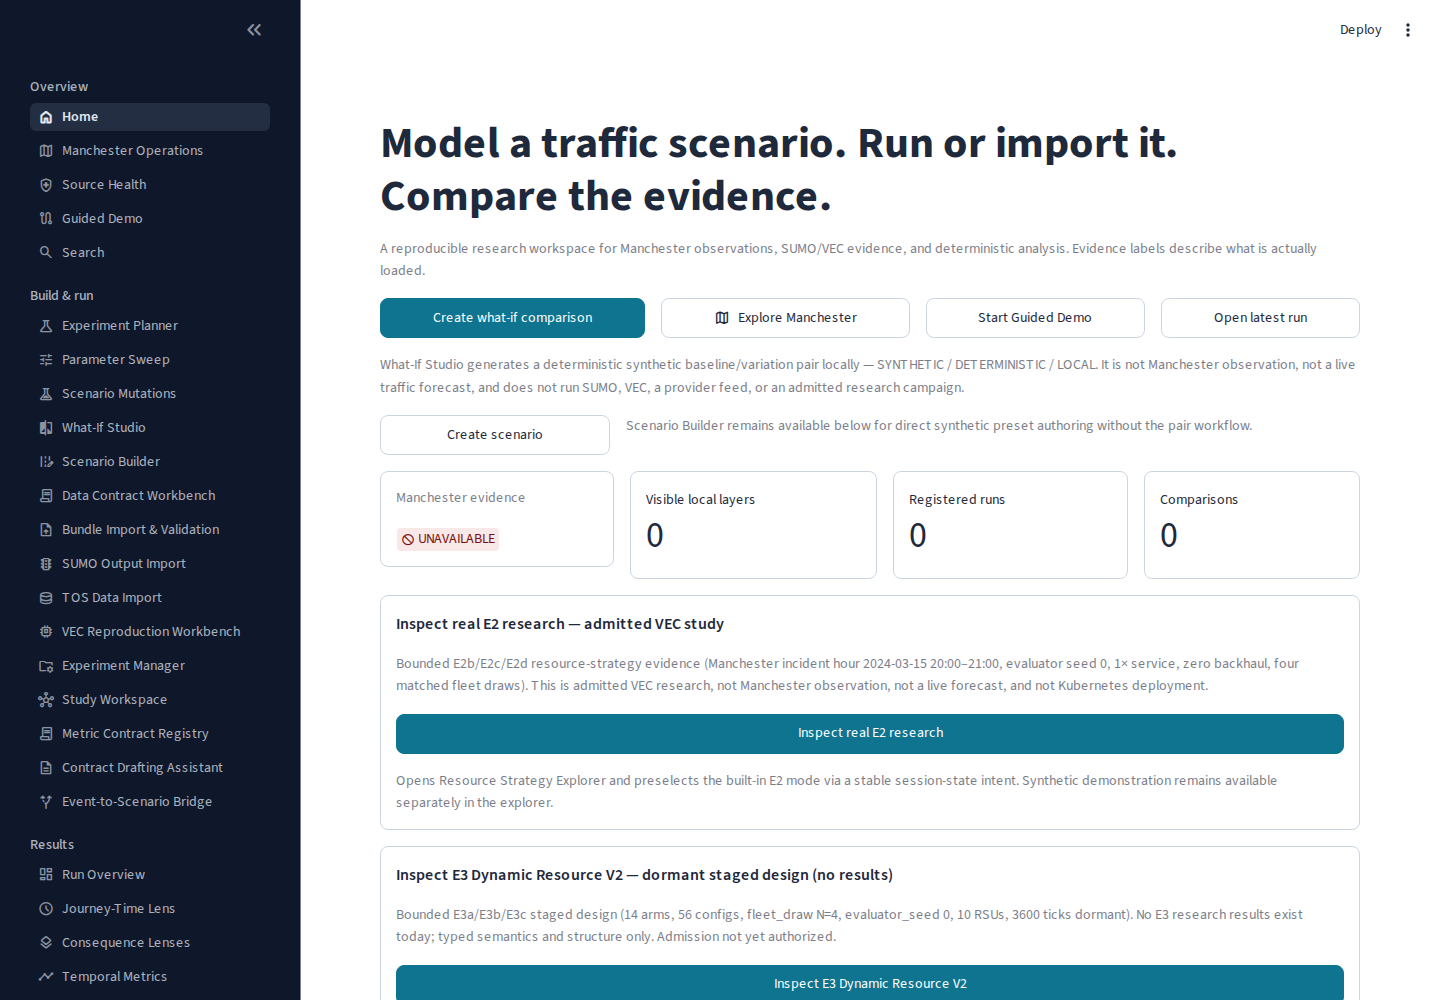
\includegraphics[width=\linewidth,height=.57\textheight,keepaspectratio]{assets/traffictwin_streamlit.png}
\caption[TrafficTwin Streamlit interface]{TrafficTwin's actual Streamlit interface captured from the pinned repository in a clean browser session; the capture receipt identifies source, route and environment. It demonstrates the software surface, not execution of the dissertation campaigns or a user-evaluation result \hyperref[source-s17]{[S17]}. Reading: use the interface to inspect and organise evidence; use the bound campaign outputs to support the numerical research claims.}\label{fig:7}
\end{figure}
% END SOURCE BLOCK 158

% BEGIN SOURCE BLOCK 159 paragraph
I designed the research questions and every evaluation experiment in this report: the E1 capacity levels, the E2b ingress-with-gate control, the E2c four-draw replication, the E2d per-task implementation and its reuse of the E2c controls, the morning pilot and its exclusion, the primary seeds, the three declared contrasts, the round-robin comparator, and the eight joint fleet/evaluator blocks with rotating arm order. The report-age levels in Section~\ref{sec:2.7} follow my supervisor's suggestion. The software was developed with generative-AI assistance: Codex and ChatGPT produced code and tooling to my specification, which I reviewed and in many cases modified before it was run (vec\_env commit 2f63706 records the per-task mode under my name). Putra supplied the actor, environment and the accounting repair \hyperref[source-s12]{[S12]}. I ran or authorised every campaign, recomputed the block-0 paired effect from the offered counts, checked the Table~\ref{tab:6} and Table~\ref{tab:7} intervals, worked through Proposition~\ref{prop:1} and Table~\ref{tab:C1}, and traced the common-target selection in the frozen evaluator source. The contribution is the formulation, design and investigation of the comparison, not the inherited software.
% END SOURCE BLOCK 159

% BEGIN SOURCE BLOCK 160 paragraph
Table~\ref{tab:10} records the limits of aggregate departures and global work with immediate reservations. Separate lifecycle fields distinguish placement, admission and success.
% END SOURCE BLOCK 160

% BEGIN SOURCE BLOCK 161 table
\begingroup
\singlespacing\footnotesize\setlength{\tabcolsep}{3pt}
\begin{xltabular}{\textwidth}{@{}YYY@{}}
\caption[Validity limits]{Validity limits and their consequences for interpretation. Reading: use each row to identify the evidence needed before extending the corresponding claim.}\label{tab:10} \\
\toprule
Limitation & Claim restricted & Consequence / evidence needed \\
\midrule\endfirsthead
\toprule
Limitation & Claim restricted & Consequence / evidence needed \\
\midrule\endhead
\bottomrule\endfoot
Batched arrivals, aggregate departures, backlog-only gate & Physical deadline feasibility & Interpret as evaluator outcomes; validate an event/transfer model against measurements \\
Global actual service work; immediate reservations & Distributed deployability & Measure estimation error and coordination delay before implementation claims \\
Original four fleet draws; new eight joint blocks on one morning trace/actor & Population uncertainty and generalisation & Joint randomness broadens stream coverage; geographical, actor and model uncertainty remain \\
Bundled scenario changes & Morning gain caused by lower density & Separate scenario analyses; factor-controlled evidence needed \\
Legacy off scoring masks differ & Admission-consistent E1 attainment and gate-only E2b attribution & Historical score intervals remain; measurement impact is not assessable from available records \\
Exact arithmetic versus float32; finite fixtures and unobserved intermediate masks & Numerical prevalence and historical causal decomposition & Two-deadline exact bound proved; constructed rounding discrepancy and reduced adverse example do not establish fleet-frequency effects \\
Two-choice spreading not evaluated & Workload-aware benefit relative to sampled placement & Run \path{dla_p2c} on the same blocks \\
Single-draw sensitivities & General staleness/forwarding robustness & Describe tested information and fixed-cost models only \\
Separately arranged raw-input access & Unrestricted full reproduction & Portable compact checks reproduce central summaries; full replay needs authorised raw inputs and preserved dependencies \\
\end{xltabular}
\endgroup
% END SOURCE BLOCK 161

% BEGIN SOURCE BLOCK 162 paragraph
Compact checks need neither actor nor JAX; full raw verification requires separately arranged access. Appendix~\ref{app:A} records access and off-machine preservation boundaries \hyperref[source-s13]{[S13]}, \hyperref[source-s16]{[S16]}.
% END SOURCE BLOCK 162

\FloatBarrier
\clearpage
% BEGIN SOURCE BLOCK 163 heading
\section{Conclusion}\label{sec:4}
% END SOURCE BLOCK 163

% BEGIN SOURCE BLOCK 164 paragraph
Under a frozen vehicle policy, common-target placement underperformed ingress while causal per-task placement exceeded it across incident, morning and joint-randomness studies. This controlled implementation comparison demonstrates the importance of destination timing and reservation visibility within established scheduling ideas.
% END SOURCE BLOCK 164

\FloatBarrier
% BEGIN SOURCE BLOCK 165 heading
\subsection{Verdict against the objectives}\label{sec:4.1}
% END SOURCE BLOCK 165

% BEGIN SOURCE BLOCK 166 table
\begingroup
\singlespacing\footnotesize\setlength{\tabcolsep}{3pt}
\begin{xltabular}{\textwidth}{@{}YYY@{}}
\caption[Objective verdicts]{Objective-by-objective verdict for the completed work. ``Met'' refers to the stated evaluator/software scope, not real-road deployment or unperformed user testing. Reading: the evidence supports the dispatch findings while leaving historical measurement impact and external validation as distinct open obligations.}\label{tab:11} \\
\toprule
Objective & Verdict & Evidence and meaning \\
\midrule\endfirsthead
\toprule
Objective & Verdict & Evidence and meaning \\
\midrule\endhead
\bottomrule\endfoot
O1 Measurement contract & Partly met & Offered/admitted/failure definitions and later authenticated checks are explicit; the historical off-mask impact remains unquantified (Section~\ref{sec:3.1}; Appendix~\ref{app:B}). \\
O2 Dispatch implementations & Met within the model & Ingress, common-target, per-task and causal cyclic contracts are operationally specified and bound to checks (Sections 2.5, 2.8 and 3.7). \\
O3 Matched estimates & Met for the sampled settings & The reversal recurs in the incident and morning samples; the separate eight-block confirmation supports all three declared contrasts (Tables 4--7). \\
O4 Mechanism and boundaries & Partly met & Destination concentration, the conditional exact bound and completed sensitivities are supported; unique causal decomposition and distributed robustness are not established (Sections 3.5--3.6; Appendix~\ref{app:C}). \\
O5 Inspectable artefact & Met for software; user benefit unassessed & Product and research components, source inventory, validation route and real interface capture are exposed (Section~\ref{sec:3.7}; Appendix~\ref{app:A}). No user study or E3 research result is claimed. \\
\end{xltabular}
\endgroup
% END SOURCE BLOCK 166

\FloatBarrier
% BEGIN SOURCE BLOCK 167 heading
\subsection{Research answers and interpretation}\label{sec:4.2}
% END SOURCE BLOCK 167

% BEGIN SOURCE BLOCK 168 paragraph
RQ1 separates comparator choice from implementation. Exploratory decomposition identified gate-enabled ingress without isolating a gate-only effect. Causal per-task placement reversed common-target's ingress ranking; separate morning samples extend support beyond adaptive incident development.
% END SOURCE BLOCK 168

% BEGIN SOURCE BLOCK 169 paragraph
RQ2 is answered by two distinct morning samples. The original four fleet draws excluded the inspected pilot and met their simultaneous-interval reversal criterion. The new eight joint fleet/evaluator blocks reproduced that result: per-task minus ingress was +4.137 percentage points and common-target minus ingress \ensuremath{-}3.504. Descriptively, the cyclic spreading step captures 84.8\% of the per-task gain over ingress, and the further workload-aware increment 15.2\%; these are arm-mean shares, not causal mechanism shares. Per-task exceeded causal round-robin by +0.631 points, with its simultaneous interval entirely positive.
% END SOURCE BLOCK 169

% BEGIN SOURCE BLOCK 170 paragraph
RQ3 is limited to the completed models. The 100 ms reports equalled fresh state; older-report changes were small under live admission and reservations. A single-draw fixed-overhead calculation retained a positive ingress advantage through 10 ms without modelling congestion or feedback. Treatment-activation checks therefore determine what these sensitivities actually test.
% END SOURCE BLOCK 170

% BEGIN SOURCE BLOCK 171 paragraph
The exact-model bound and gate/service/drain assumptions explain recurring destinations, within Appendix~\ref{app:C}'s numerical limits. Four-draw descriptive accounting locates most gains in reduced rejection, alongside recovered admitted misses and smaller losses; it does not identify task-level causal effects.
% END SOURCE BLOCK 171

\FloatBarrier
% BEGIN SOURCE BLOCK 172 heading
\subsection{Prioritised future work}\label{sec:4.3}
% END SOURCE BLOCK 172

% BEGIN SOURCE BLOCK 173 paragraph
First, I would evaluate \path{dla_p2c} on the sealed eight blocks under identical controls, to separate randomised sampling from exact least-workload selection. This post-hoc addition would be outside the sealed family.
% END SOURCE BLOCK 173

% BEGIN SOURCE BLOCK 174 paragraph
Second, an event-level service and communication model should be checked against measured timing, including transfers and individual departures. Simulation verification and VEC communication/resource models provide the relevant foundation \cite{ref12}, \cite{ref17}, \cite{ref18}. The decisive test would be whether the reversal survives a calibrated timing model, not whether another abstract queue simulation produces more significant digits.
% END SOURCE BLOCK 174

% BEGIN SOURCE BLOCK 175 paragraph
Third, I would separate imperfect workload estimates, acknowledgement delay and admission policy, following imperfect-information routing and digital-twin estimation models \cite{ref10}, \cite{ref16}. This tests how live admission protects placement based on older reports.
% END SOURCE BLOCK 175

% BEGIN SOURCE BLOCK 176 paragraph
Fourth, I would test independently selected traces and actors under prospective controls and seed-level reporting \cite{ref5}, \cite{ref6}, \cite{ref19}. Action masking and V2V-helper selection need separate studies \cite{ref22}, \cite{ref23}; product user evaluation requires its own protocol.
% END SOURCE BLOCK 176

% BEGIN SOURCE BLOCK 177 paragraph
Within the studied evaluator and matched populations, implementation semantics reverse the ingress comparison, and workload-aware causal placement improves attainment over the tested spreading rule.
% END SOURCE BLOCK 177

\FloatBarrier
% BEGIN SOURCE BLOCK 178 heading
\subsection{Reflection on the process}\label{sec:4.4}
% END SOURCE BLOCK 178

% BEGIN SOURCE BLOCK 179 paragraph
I learned that an adaptive experiment can identify a useful next question without providing independent confirmation of its answer. E2c made the negative common-target comparison repeatable across fleet draws. I then designed E2d to change target timing and reservation visibility while reusing the E2c controls. That reuse made the comparison efficient and interpretable, but the inspected result had already influenced my choice of intervention. I therefore needed prospective replication with declared inputs and contrasts. I excluded the morning pilot from primary inference, and the later sealed joint blocks gave the additional comparator a separate, explicit evidence boundary.
% END SOURCE BLOCK 179

% BEGIN SOURCE BLOCK 180 paragraph
I also narrowed the project as the work developed. I dropped the planned user evaluation, so product functionality and browser checks cannot establish usability or operator benefit. E3 remained unexecuted; implemented interfaces and campaign preparation did not supply research results. These decisions concentrated the report on a comparison I could support, while leaving different questions to their own protocols. In hindsight, I should have made the evaluator's existing two-choice option more prominent when explaining comparator selection.
% END SOURCE BLOCK 180

% BEGIN SOURCE BLOCK 181 paragraph
Raw-data retention was another practical lesson. Summaries and receipts preserve the reported historical intervals, but they cannot answer every later question about task-level scoring. I should have planned retention around future audit needs as well as immediate analysis. The retained September inventory improves traceability, while an independently verified off-machine copy and examiner access still require completion.
% END SOURCE BLOCK 181

% BEGIN SOURCE BLOCK 182 paragraph
I controlled AI assistance through specifications, code review, personal modification and campaign boundaries. Codex and ChatGPT helped generate implementation and text; I remained responsible for deciding what matched my design and what entered the report. Sealed controls and deterministic receipts made execution inspectable, while my completed author checks addressed my understanding. This experience reinforced the need to record design decisions, supplied code, automated assistance and personal verification separately throughout the work.
% END SOURCE BLOCK 182

% BEGIN SOURCE BLOCK 183 bibliography_open
\clearpage\singlespacing\addcontentsline{toc}{section}{References}\begin{thebibliography}{99}
% END SOURCE BLOCK 183

% BEGIN SOURCE BLOCK 184 bibliography_item
\bibitem{ref1} Y. Mao, C. You, J. Zhang, K. Huang and K. B. Letaief. ``A Survey on Mobile Edge Computing: The Communication Perspective.'' \emph{IEEE Communications Surveys \& Tutorials}, 19(4), 2322--2358, 2017. DOI: 10.1109/COMST.2017.2745201. \href{\detokenize{https://arxiv.org/abs/1701.01090}}{Author manuscript}.
% END SOURCE BLOCK 184

% BEGIN SOURCE BLOCK 185 bibliography_item
\bibitem{ref2} M. Harchol-Balter, M. E. Crovella and C. D. Murta. ``On Choosing a Task Assignment Policy for a Distributed Server System.'' \emph{Computer Performance Evaluation (TOOLS 1998)}, LNCS 1469, 231--242, 1998. DOI: 10.1007/3-540-68061-6\_19. \href{\detokenize{https://www.cs.cmu.edu/~harchol/Papers/tools.pdf}}{Author manuscript}.
% END SOURCE BLOCK 185

% BEGIN SOURCE BLOCK 186 bibliography_item
\bibitem{ref3} J. Schulman, F. Wolski, P. Dhariwal, A. Radford and O. Klimov. ``Proximal Policy Optimization Algorithms.'' arXiv:1707.06347, 2017. \href{\detokenize{https://arxiv.org/abs/1707.06347}}{Author manuscript}.
% END SOURCE BLOCK 186

% BEGIN SOURCE BLOCK 187 bibliography_item
\bibitem{ref4} C. Yu, A. Velu, E. Vinitsky, J. Gao, Y. Wang, A. Bayen and Y. Wu. ``The Surprising Effectiveness of PPO in Cooperative Multi-Agent Games.'' \emph{Advances in Neural Information Processing Systems}, 35, 24611--24624, 2022. \href{\detokenize{https://papers.nips.cc/paper/2022/file/9c1535a02f0ce079433344e14d910597-Paper-Datasets_and_Benchmarks.pdf}}{Proceedings paper}.
% END SOURCE BLOCK 187

% BEGIN SOURCE BLOCK 188 bibliography_item
\bibitem{ref5} P. Henderson, R. Islam, P. Bachman, J. Pineau, D. Precup and D. Meger. ``Deep Reinforcement Learning That Matters.'' \emph{Proceedings of the AAAI Conference on Artificial Intelligence}, 32(1), 2018. DOI: 10.1609/aaai.v32i1.11694. \href{\detokenize{https://ojs.aaai.org/index.php/AAAI/article/view/11694}}{Publisher record}.
% END SOURCE BLOCK 188

% BEGIN SOURCE BLOCK 189 bibliography_item
\bibitem{ref6} R. Agarwal, M. Schwarzer, P. S. Castro, A. Courville and M. G. Bellemare. ``Deep Reinforcement Learning at the Edge of the Statistical Precipice.'' \emph{Advances in Neural Information Processing Systems}, 34, 29304--29320, 2021. \href{\detokenize{https://proceedings.neurips.cc/paper/2021/hash/f514cec81cb148559cf475e7426eed5e-Abstract.html}}{Proceedings record}.
% END SOURCE BLOCK 189

% BEGIN SOURCE BLOCK 190 bibliography_item
\bibitem{ref7} R. Gorsane, O. Mahjoub, R. de Kock, R. Dubb, S. Singh and A. Pretorius. ``Towards a Standardised Performance Evaluation Protocol for Cooperative MARL.'' \emph{Advances in Neural Information Processing Systems}, 35, 5510--5521, 2022. \href{\detokenize{https://arxiv.org/abs/2209.10485}}{Author manuscript}.
% END SOURCE BLOCK 190

% BEGIN SOURCE BLOCK 191 bibliography_item
\bibitem{ref8} P. Alvarez Lopez, M. Behrisch, L. Bieker-Walz, J. Erdmann, Y.-P. Flötteröd, R. Hilbrich, L. Lücken, J. Rummel, P. Wagner and E. Wießner. ``Microscopic Traffic Simulation using SUMO.'' \emph{21st International Conference on Intelligent Transportation Systems (ITSC)}, 2575--2582, 2018. DOI: 10.1109/ITSC.2018.8569938. \href{\detokenize{https://elib.dlr.de/127994/}}{DLR author repository}.
% END SOURCE BLOCK 191

% BEGIN SOURCE BLOCK 192 bibliography_item
\bibitem{ref9} K. Ousterhout, P. Wendell, M. Zaharia and I. Stoica. ``Sparrow: Distributed, Low Latency Scheduling.'' \emph{24th ACM Symposium on Operating Systems Principles}, 69--84, 2013. DOI: 10.1145/2517349.2522716. \href{\detokenize{https://sigops.org/s/conferences/sosp/2013/papers/p69-ousterhout.pdf}}{Proceedings paper}.
% END SOURCE BLOCK 192

% BEGIN SOURCE BLOCK 193 bibliography_item
\bibitem{ref10} S. Vargaftik, I. Keslassy and A. Orda. ``LSQ: Load Balancing in Large-Scale Heterogeneous Systems With Multiple Dispatchers.'' \emph{IEEE/ACM Transactions on Networking}, 28(3), 1186--1198, 2020. DOI: 10.1109/TNET.2020.2980061. \href{\detokenize{https://webee.technion.ac.il/~isaac/p/ton20_lsq.pdf}}{Author manuscript}.
% END SOURCE BLOCK 193

% BEGIN SOURCE BLOCK 194 bibliography_item
\bibitem{ref11} J. Niño-Mora. ``Admission and routing of soft real-time jobs to multiclusters: Design and comparison of index policies.'' \emph{Computers \& Operations Research}, 39, 3431--3444, 2012. DOI: 10.1016/j.cor.2012.05.004. \href{\detokenize{https://arxiv.org/abs/2207.12815}}{Author manuscript, deposited 2022}.
% END SOURCE BLOCK 194

% BEGIN SOURCE BLOCK 195 bibliography_item
\bibitem{ref12} R. G. Sargent. ``Verification and Validation of Simulation Models.'' \emph{Proceedings of the 2011 Winter Simulation Conference}, 183--198, 2011. \href{\detokenize{https://www.informs-sim.org/wsc11papers/016.pdf}}{Proceedings paper}.
% END SOURCE BLOCK 195

% BEGIN SOURCE BLOCK 196 bibliography_item
\bibitem{ref13} L. Ying, R. Srikant and X. Kang. ``The Power of Slightly More than One Sample in Randomized Load Balancing.'' \emph{IEEE INFOCOM}, 1131--1139, 2015. \href{\detokenize{https://doi.org/10.1109/INFOCOM.2015.7218487}}{doi:10.1109/INFOCOM.2015.7218487}. \href{\detokenize{https://bpb-us-w2.wpmucdn.com/sites.coecis.cornell.edu/dist/9/287/files/2019/08/Srikant-1-YinSriKan14tech.pdf}}{Author technical manuscript}.
% END SOURCE BLOCK 196

% BEGIN SOURCE BLOCK 197 bibliography_item
\bibitem{ref14} JAX authors. ``Benchmarking JAX code.'' Official JAX documentation, accessed 8 September 2026. \href{\detokenize{https://docs.jax.dev/en/latest/benchmarking.html}}{Benchmarking guidance}. Used for timing procedure, not scheduler efficacy.
% END SOURCE BLOCK 197

% BEGIN SOURCE BLOCK 198 bibliography_item
\bibitem{ref15} S. Dasgupta, M. Rahman, A. D. Lidbe, W. Lu and S. Jones. ``A Transportation Digital-Twin Approach for Adaptive Traffic Control Systems.'' arXiv:2109.10863, 2021. \href{\detokenize{https://arxiv.org/abs/2109.10863}}{Source}.
% END SOURCE BLOCK 198

% BEGIN SOURCE BLOCK 199 bibliography_item
\bibitem{ref16} Y. Xie, Q. Wu and P. Fan. ``Digital Twin Vehicular Edge Computing Network: Task Offloading and Resource Allocation.'' arXiv:2407.11310, 2024. \href{\detokenize{https://arxiv.org/abs/2407.11310}}{Source}.
% END SOURCE BLOCK 199

% BEGIN SOURCE BLOCK 200 bibliography_item
\bibitem{ref17} S. Cho, S. I. Choi, S. H. Oh, I. P. Roberts and S. H. Lee. ``Autonomous Task Offloading of Vehicular Edge Computing with Parallel Computation Queues.'' \emph{IEEE Transactions on Mobile Computing}, 25(5), 7166--7181, 2026. DOI: 10.1109/TMC.2025.3640244. Author version arXiv:2509.03935v2. \href{\detokenize{https://arxiv.org/abs/2509.03935v2}}{Source}.
% END SOURCE BLOCK 200

% BEGIN SOURCE BLOCK 201 bibliography_item
\bibitem{ref18} Q. Wu, W. Wang, P. Fan, Q. Fan, J. Wang and K. B. Letaief. ``URLLC-Awared Resource Allocation for Heterogeneous Vehicular Edge Computing.'' arXiv:2311.18352, 2023. \href{\detokenize{https://arxiv.org/abs/2311.18352}}{Source}.
% END SOURCE BLOCK 201

% BEGIN SOURCE BLOCK 202 bibliography_item
\bibitem{ref19} J. Pineau, P. Vincent-Lamarre, K. Sinha, V. Larivière, A. Beygelzimer, F. d'Alché-Buc, E. Fox and H. Larochelle. ``Improving Reproducibility in Machine Learning Research (A Report from the NeurIPS 2019 Reproducibility Program).'' \emph{Journal of Machine Learning Research}, 22(164), 1--20, 2021. \href{\detokenize{https://jmlr.org/papers/v22/20-303.html}}{Source}.
% END SOURCE BLOCK 202

% BEGIN SOURCE BLOCK 203 bibliography_item
\bibitem{ref20} G. Wilson et al. ``Best Practices for Scientific Computing.'' \emph{PLOS Biology}, 12(1), e1001745, 2014. DOI: 10.1371/journal.pbio.1001745. \href{\detokenize{https://journals.plos.org/plosbiology/article?id=10.1371/journal.pbio.1001745}}{Source}.
% END SOURCE BLOCK 203

% BEGIN SOURCE BLOCK 204 bibliography_item
\bibitem{ref21} G. K. Sandve, A. Nekrutenko, J. Taylor and E. Hovig. ``Ten Simple Rules for Reproducible Computational Research.'' \emph{PLOS Computational Biology}, 9(10), e1003285, 2013. DOI: 10.1371/journal.pcbi.1003285. \href{\detokenize{https://journals.plos.org/ploscompbiol/article?id=10.1371/journal.pcbi.1003285}}{Source}.
% END SOURCE BLOCK 204

% BEGIN SOURCE BLOCK 205 bibliography_item
\bibitem{ref22} E. Krijestorac, A. Memedi, T. Higuchi, S. Ucar, O. Altintas and D. Cabric. ``Hybrid Vehicular and Cloud Distributed Computing: A Case for Cooperative Perception.'' arXiv:2010.05693, 2020. \href{\detokenize{https://arxiv.org/abs/2010.05693}}{Source}.
% END SOURCE BLOCK 205

% BEGIN SOURCE BLOCK 206 bibliography_item
\bibitem{ref23} S. Huang and S. Ontañón. ``A Closer Look at Invalid Action Masking in Policy Gradient Algorithms.'' arXiv:2006.14171, 2020. \href{\detokenize{https://arxiv.org/abs/2006.14171}}{Source}.
% END SOURCE BLOCK 206

% BEGIN SOURCE BLOCK 207 bibliography_item
\bibitem{ref24} W. Fan, Y. Zhang, G. Zhou and Y. Liu. ``Deep Reinforcement Learning-Based Task Offloading for Vehicular Edge Computing With Flexible RSU-RSU Cooperation.'' \emph{IEEE Transactions on Intelligent Transportation Systems}, 25(7), 7712--7725, 2024. DOI: 10.1109/TITS.2024.3349546. \href{\detokenize{https://doi.org/10.1109/TITS.2024.3349546}}{Source}.
% END SOURCE BLOCK 207

% BEGIN SOURCE BLOCK 208 bibliography_item
\bibitem{ref25} W. Fan, Y. Yu, C. Bao and Y. Liu. ``Vehicular Edge Intelligence: DRL-Based Resource Orchestration for Task Inference in Vehicle-RSU-Edge Collaborative Networks.'' \emph{IEEE Transactions on Mobile Computing}, 24(10), 10927--10944, 2025. DOI: 10.1109/TMC.2025.3572296. \href{\detokenize{https://doi.org/10.1109/TMC.2025.3572296}}{Source}.
% END SOURCE BLOCK 208

% BEGIN SOURCE BLOCK 209 bibliography_close
\end{thebibliography}
% END SOURCE BLOCK 209

% BEGIN SOURCE BLOCK 210 appendix_open
\appendix
\renewcommand{\thetable}{\Alph{section}\arabic{table}}
% END SOURCE BLOCK 210

% BEGIN SOURCE BLOCK 211 heading
\appendixsection{app:A}{Evidence sources and reproducibility}
% END SOURCE BLOCK 211

% BEGIN SOURCE BLOCK 212 paragraph
The sources below are project evidence, separate from scholarly references. Relative links resolve in the repository checkout. The \href{\detokenize{https://github.com/Abdulla4akash/traffictwin/tree/04f3b6a95c7bc06c80ed95b54762f12861bba183}}{historical baseline} and later packages retain their respective source identities. The current \href{\detokenize{CLAIM_SOURCE_MAP.md}}{claim-to-source map} records support and limits.
% END SOURCE BLOCK 212

% BEGIN SOURCE BLOCK 213 anchor
\phantomsection\label{source-s0}
% END SOURCE BLOCK 213

% BEGIN SOURCE BLOCK 214 paragraph
\textbf{S0 --- Accounting validity.} \href{\detokenize{../../evaluation/vec_followup_2026-09-07/historical_e0_e2d/experiments/E0/README.md}}{E0 report and evidence}. Full evidence commit \path{29d8945862b7df1bd5d7879ba1d980a388f6be0d}.
% END SOURCE BLOCK 214

% BEGIN SOURCE BLOCK 215 anchor
\phantomsection\label{source-s1}
% END SOURCE BLOCK 215

% BEGIN SOURCE BLOCK 216 paragraph
\textbf{S1 --- Waiting-room capacity.} \href{\detokenize{../../evaluation/vec_followup_2026-09-07/historical_e0_e2d/experiments/E1/README.md}}{E1 report}, with five-draw comparison and validation records.
% END SOURCE BLOCK 216

% BEGIN SOURCE BLOCK 217 anchor
\phantomsection\label{source-s2}
% END SOURCE BLOCK 217

% BEGIN SOURCE BLOCK 218 paragraph
\textbf{S2 --- Exploratory admission/placement decomposition.} \href{\detokenize{../../evaluation/vec_followup_2026-09-07/historical_e0_e2d/experiments/E2b/README.md}}{E2b report and factorial evidence}.
% END SOURCE BLOCK 218

% BEGIN SOURCE BLOCK 219 anchor
\phantomsection\label{source-s3}
% END SOURCE BLOCK 219

% BEGIN SOURCE BLOCK 220 paragraph
\textbf{S3 --- Incident replication and reversal.} \href{\detokenize{../../evaluation/vec_followup_2026-09-07/historical_e0_e2d/experiments/E2c/README.md}}{E2c report} and \href{\detokenize{../../evaluation/vec_followup_2026-09-07/historical_e0_e2d/experiments/E2d/README.md}}{E2d report}. Frozen E2d evaluator commit \path{2f63706f46319433a2ba3af1df97afd0e56a95d1}; exact E2c controls reused.
% END SOURCE BLOCK 220

% BEGIN SOURCE BLOCK 221 anchor
\phantomsection\label{source-s4}
% END SOURCE BLOCK 221

% BEGIN SOURCE BLOCK 222 paragraph
\textbf{S4 --- Experimental architecture and implementation.} \href{\detokenize{../../evaluation/vec_followup_2026-09-07/historical_e0_e2d/docs/METHODOLOGY.md}}{Frozen method}, \href{\detokenize{../../evaluation/vec_followup_2026-09-07/frozen_evaluator/eval/e2d_per_task_placement.py}}{per-task source}, \href{\detokenize{../../evaluation/vec_followup_2026-09-07/frozen_evaluator/eval/eval_sumo_stage1_mc.py}}{evaluator source}, \href{\detokenize{../empirical_extension_2026-09-08/experimental/vendor/vec_jax.py}}{environment source}, and \href{\detokenize{../../correspondence/sandra_randy_vec_progress_email_thread_2026-08-18.md}}{implementation correspondence}, PDF pages 1--2 for Putra's confirmations.
% END SOURCE BLOCK 222

% BEGIN SOURCE BLOCK 223 anchor
\phantomsection\label{source-s5}
% END SOURCE BLOCK 223

% BEGIN SOURCE BLOCK 224 paragraph
\textbf{S5 --- State-information sensitivity.} \href{\detokenize{../../evaluation/vec_followup_2026-09-07/frozen_evaluator/docs/RSU_STATE_DELAY.md}}{Timing contract}, \href{\detokenize{../../evaluation/vec_followup_2026-09-07/state-delay-pilot-2026-09-07/comparison.csv}}{five-cell comparison} and \href{\detokenize{../../evaluation/vec_followup_2026-09-07/state-delay-pilot-2026-09-07/mechanism_audit.json}}{report-state audit}.
% END SOURCE BLOCK 224

% BEGIN SOURCE BLOCK 225 anchor
\phantomsection\label{source-s6}
% END SOURCE BLOCK 225

% BEGIN SOURCE BLOCK 226 paragraph
\textbf{S6 --- Forwarding sensitivity.} \href{\detokenize{../../evaluation/vec_followup_2026-09-07/forwarding-sensitivity-2026-09-07/qualification.json}}{Qualification}, \href{\detokenize{../../evaluation/vec_followup_2026-09-07/forwarding-sensitivity-2026-09-07/forwarding_sensitivity.csv}}{outcomes} and \href{\detokenize{../../evaluation/vec_followup_2026-09-07/forwarding-sensitivity-2026-09-07/analysis_validation.json}}{analysis validation}.
% END SOURCE BLOCK 226

% BEGIN SOURCE BLOCK 227 anchor
\phantomsection\label{source-s7}
% END SOURCE BLOCK 227

% BEGIN SOURCE BLOCK 228 paragraph
\textbf{S7 --- Morning exploratory pilot.} \href{\detokenize{../../evaluation/vec_followup_2026-09-07/generalisation-pilot-2026-09-07/RESULTS.md}}{Results} and \href{\detokenize{../../evaluation/vec_followup_2026-09-07/generalisation-pilot-2026-09-07/input_validation.json}}{canonical input validation}.
% END SOURCE BLOCK 228

% BEGIN SOURCE BLOCK 229 anchor
\phantomsection\label{source-s8}
% END SOURCE BLOCK 229

% BEGIN SOURCE BLOCK 230 paragraph
\textbf{S8 --- Morning primary replication.} \href{\detokenize{../../evaluation/vec_followup_2026-09-07/generalisation-replication-2026-09-07/PROTOCOL.md}}{Protocol}, \href{\detokenize{../../evaluation/vec_followup_2026-09-07/generalisation-replication-2026-09-07/manifest.json}}{manifest}, \href{\detokenize{../../evaluation/vec_followup_2026-09-07/generalisation-replication-2026-09-07/paired_differences.csv}}{paired differences} and \href{\detokenize{../../evaluation/vec_followup_2026-09-07/generalisation-replication-2026-09-07/paired_intervals.csv}}{paired intervals}. Full follow-up evaluator commit \path{908bd10f86542de94fc38af90dd56c2ccc08cf9b}.
% END SOURCE BLOCK 230

% BEGIN SOURCE BLOCK 231 anchor
\phantomsection\label{source-s9}
% END SOURCE BLOCK 231

% BEGIN SOURCE BLOCK 232 paragraph
\textbf{S9 --- Five-RSU mechanism audit.} \href{\detokenize{../../evaluation/common_target_mechanism_audit_2026-09-07/evidence/REPORT.md}}{Completed post-hoc report} and \href{\detokenize{../../evaluation/common_target_mechanism_audit_2026-09-07/evidence/audit_results.json}}{audit results with input identities}.
% END SOURCE BLOCK 232

% BEGIN SOURCE BLOCK 233 anchor
\phantomsection\label{source-s10}
% END SOURCE BLOCK 233

% BEGIN SOURCE BLOCK 234 paragraph
\textbf{S10 --- Unrun falsification proposal.} \href{\detokenize{../../evaluation/common_target_mechanism_audit_2026-09-07/TIEBREAK_PREFIX_PROPOSAL.md}}{Rotating-tie-break prefix protocol}.
% END SOURCE BLOCK 234

% BEGIN SOURCE BLOCK 235 anchor
\phantomsection\label{source-s11}
% END SOURCE BLOCK 235

% BEGIN SOURCE BLOCK 236 paragraph
\textbf{S11 --- Artifact and preservation.} \href{\detokenize{../../architecture_current_release.md}}{Product architecture}, \href{\detokenize{../../quality/final_release_status_20260815.md}}{release/execution boundary}, \href{\detokenize{../../evaluation/vec_followup_2026-09-07/ARCHIVE_INVENTORY.json}}{evidence archive inventory} and \href{\detokenize{../../evaluation/vec_followup_2026-09-07/COMPACT_VERIFICATION.json}}{compact verification receipt}. The separate E3 Dynamic Resource V2 campaign remains unexecuted.
% END SOURCE BLOCK 236

% BEGIN SOURCE BLOCK 237 anchor
\phantomsection\label{source-s12}
% END SOURCE BLOCK 237

% BEGIN SOURCE BLOCK 238 paragraph
\textbf{S12 --- Contribution and repair history.} Read-only inspection of \path{vec_env} commits \href{\detokenize{https://github.com/Abdulla4akash/vec_env/commit/4cb7c06aab1b455d68f71ea9143172463784dea9}}{4cb7c06}, \href{\detokenize{https://github.com/Abdulla4akash/vec_env/commit/0f01f4d2082d3e8b735e74a873095ab8eeba37cc}}{0f01f4d} and \href{\detokenize{https://github.com/Abdulla4akash/vec_env/commit/2f63706f46319433a2ba3af1df97afd0e56a95d1}}{2f63706}, and TrafficTwin \href{\detokenize{https://github.com/Abdulla4akash/traffictwin/blob/29d8945862b7df1bd5d7879ba1d980a388f6be0d/tests/test_validate_e0_smoke.py}}{E0 validation tests at 29d894}. Source comments explicitly credit my questions; my \href{\detokenize{AUTHOR_ACTIONS.md}}{15 September confirmation} records my design, implementation changes and completed verification.
% END SOURCE BLOCK 238

% BEGIN SOURCE BLOCK 239 anchor
\phantomsection\label{source-s13}
% END SOURCE BLOCK 239

% BEGIN SOURCE BLOCK 240 paragraph
\textbf{S13 --- Retrospective gap closure, 8 September 2026.} The \href{\detokenize{../gap_closure_2026-09-08/verification/README.md}}{verification entry point} documents the field contract, source bindings, 87-file authentication, 19-run audit, \href{\detokenize{../gap_closure_2026-09-08/verification/results/OUTCOME_TRANSITIONS.json}}{23 paired transitions}, \href{\detokenize{../gap_closure_2026-09-08/verification/results/KERNEL_RESULTS.json}}{440-case reference} and production comparison. These completed checks and their historical sources remain unchanged.
% END SOURCE BLOCK 240

% BEGIN SOURCE BLOCK 241 anchor
\phantomsection\label{source-s14}
% END SOURCE BLOCK 241

% BEGIN SOURCE BLOCK 242 paragraph
\textbf{S14 --- Production-domain mechanism analysis.} \href{\detokenize{../production_mechanism_2026-09-08/analysis/MATHEMATICS.md}}{Model and proof}, \href{\detokenize{../production_mechanism_2026-09-08/analysis/PROTOCOL.md}}{initial diagnostic protocol}, \href{\detokenize{../production_mechanism_2026-09-08/analysis/FOLLOWUP_PROTOCOL.md}}{bounded follow-up protocol}, \href{\detokenize{../production_mechanism_2026-09-08/analysis/diagnostics.py}}{executable diagnostics}, \href{\detokenize{../production_mechanism_2026-09-08/analysis/results/DIAGNOSTICS.json}}{full results}, \href{\detokenize{../production_mechanism_2026-09-08/analysis/results/NUMERICAL_FOLLOWUP.json}}{numerical follow-up}, \href{\detokenize{../production_mechanism_2026-09-08/analysis/results/ADVERSE_PRODUCTION.json}}{adverse example and helper checks}, \href{\detokenize{../production_mechanism_2026-09-08/analysis/results/DIMENSION_CHECK.json}}{dimension checks} and \href{\detokenize{../production_mechanism_2026-09-08/analysis/results/OUTCOME_ACCOUNTING.json}}{outcome accounting}. This is retrospective analysis added after the completed experiments and gap closure.
% END SOURCE BLOCK 242

% BEGIN SOURCE BLOCK 243 anchor
\phantomsection\label{source-s15}
% END SOURCE BLOCK 243

% BEGIN SOURCE BLOCK 244 paragraph
\textbf{S15 --- Retrospective empirical/engineering extension.} \href{\detokenize{../empirical_extension_2026-09-08/analysis/PROTOCOL.md}}{Declared analysis protocol}, \href{\detokenize{../empirical_extension_2026-09-08/analysis/results/TASK_TYPES.json}}{task-type counts and bindings}, \href{\detokenize{../empirical_extension_2026-09-08/analysis/benchmark.py}}{benchmark implementation} and \href{\detokenize{../empirical_extension_2026-09-08/analysis/results/BENCHMARK.json}}{measured results}, \href{\detokenize{../empirical_extension_2026-09-08/experimental/round_robin.py}}{cyclic implementation}, \href{\detokenize{../empirical_extension_2026-09-08/analysis/results/COMPATIBILITY_TESTS.json}}{compatibility evidence}, \href{\detokenize{../empirical_extension_2026-09-08/confirmation/PROTOCOL.md}}{sealed confirmation protocol}, \href{\detokenize{../empirical_extension_2026-09-08/confirmation/DRY_RUN.json}}{dry-run receipt}, and \href{\detokenize{../empirical_extension_2026-09-08/README.md}}{verification route}. That original preparation package remains disabled and unchanged; S16 records the separately authorised execution.
% END SOURCE BLOCK 244

% BEGIN SOURCE BLOCK 245 anchor
\phantomsection\label{source-s16}
% END SOURCE BLOCK 245

% BEGIN SOURCE BLOCK 246 paragraph
\textbf{S16 --- Authorised joint-randomness confirmation.} \href{\detokenize{../joint_confirmation_2026-09-08/confirmation/EXECUTION_AMENDMENT.md}}{Execution amendment}, \href{\detokenize{../joint_confirmation_2026-09-08/confirmation/PROTOCOL_EXECUTION.md}}{qualified execution protocol}, \href{\detokenize{../joint_confirmation_2026-09-08/confirmation/SEALED_EXECUTION.json}}{execution seal}, \href{\detokenize{../joint_confirmation_2026-09-08/experimental/evaluator_v2.py}}{versioned evaluator}, \href{\detokenize{../joint_confirmation_2026-09-08/confirmation/runner.py}}{runner and completion gate}, \href{\detokenize{../joint_confirmation_2026-09-08/confirmation/validation.py}}{task/queue/block validation}, \href{\detokenize{../joint_confirmation_2026-09-08/confirmation/analyse.py}}{sealed analysis}, \href{\detokenize{../joint_confirmation_2026-09-08/evidence/QUALIFICATION.json}}{qualification receipt}, \href{\detokenize{../joint_confirmation_2026-09-08/evidence/QUALIFICATION_FOLLOWUP.json}}{prelaunch safeguard checks}, and \href{\detokenize{../joint_confirmation_2026-09-08/README.md}}{verification/access route}. \href{\detokenize{../joint_confirmation_2026-09-08/evidence/ANALYSIS.json}}{Completed primary analysis}, \href{\detokenize{../joint_confirmation_2026-09-08/evidence/CELL_RESULTS.csv}}{all cell counts}, \href{\detokenize{../joint_confirmation_2026-09-08/evidence/BLOCK_CONTROLS.json}}{block controls} and \href{\detokenize{../joint_confirmation_2026-09-08/evidence/RAW_INVENTORY.json}}{raw inventory} bind the new results. This study is separate from the original four-draw sample, pilot and retrospective analyses.
% END SOURCE BLOCK 246

% BEGIN SOURCE BLOCK 247 paragraph
The runtime is CPython 3.11.15, JAX/JAXlib 0.4.30 and NumPy 1.26.4, CPU, x64 disabled. Historical manifests retain their own identities. Full reproduction also needs the frozen actor, traces and authorised inputs.
% END SOURCE BLOCK 247

% BEGIN SOURCE BLOCK 248 anchor
\phantomsection\label{source-s17}
% END SOURCE BLOCK 248

% BEGIN SOURCE BLOCK 249 paragraph
\textbf{S17 --- Examiner-revision artefact evidence.} The \href{\detokenize{evidence/ARTEFACT_INVENTORY.json}}{source inventory}, \href{\detokenize{evidence/COMPACT_CHECKS.json}}{compact recomputation}, \href{\detokenize{evidence/DESCRIPTIVE_SPLIT.json}}{descriptive split}, \href{\detokenize{evidence/RSU_LAYOUT.json}}{figure inputs} and \href{\detokenize{document/REVISION_VALIDATION.json}}{revision validation} are generated from the pinned repository without new research execution. The \href{\detokenize{README.md}}{revision record} distinguishes historical receipts, fresh document checks, actual browser capture and author-only completion items. The manuscript's source base is \path{1e01b755b8b633f43c9c7bb6fdd0d75beb6469e8}.
% END SOURCE BLOCK 249

% BEGIN SOURCE BLOCK 250 heading
\appendixsection{app:B}{Audit coverage and diagnostic boundaries}
% END SOURCE BLOCK 250

% BEGIN SOURCE BLOCK 251 paragraph
Table~\ref{tab:B1} retains the completed gap-closure audit coverage. Those raw checks and joins were not repeated for this revision.
% END SOURCE BLOCK 251

% BEGIN SOURCE BLOCK 252 table
\begingroup
\singlespacing\footnotesize\setlength{\tabcolsep}{3pt}
\begin{xltabular}{\textwidth}{@{}YYYY@{}}
\caption[Historical audit coverage]{Historical availability and retained gap-closure audit coverage, 8 September 2026. Historical receipts remain unchanged. Reading: distinguish archived summaries from raw-array audit coverage and retain unquantifiable historical scoring impact.}\label{tab:B1} \\
\toprule
Records & Available evidence / coverage & Completed gap-closure checks & Consequence \\
\midrule\endfirsthead
\toprule
Records & Available evidence / coverage & Completed gap-closure checks & Consequence \\
\midrule\endhead
\bottomrule\endfoot
E0: two ten-step repeats and full seed 0 & Surviving receipts, manifests, sources; full receipt records 834,120 cap rejections & Not assessable from available records & Raw arrays not retained; summaries and receipts archived \\
E1: five seeds \ensuremath{\times} three caps & Fifteen run summaries/receipts; seed-0 middle cap reuses E0 & Not assessable from available records & Original interval reproduced from summaries; scoring impact unresolved \\
E2 off/jsq/dla seed 0 and E2b reused cells & Hash-bound summaries and receipts; E2b reuses E2 exactly & Not assessable from available records & No new cell or historical task join inferred from reuse \\
E2b new ingress / E2c / E2d originals & Compact sources/records survive; original raw availability not established & Not assessable from available records & No non-retention or fresh raw-validation claim extended to these studies \\
September morning primary & Twelve full runs, seeds 0/2/3/4; 1,744,116 offered per cell & Zero discrepancies in each inspected run & Supports these gate-enabled records; excludes pilot from inference \\
September morning pilot & Two full seed-1 runs, 1,744,116 offered each & Zero discrepancies in each inspected run & Remains exploratory, outside primary inference \\
September incident sensitivity pilot & Five full seed-1 runs, 13,076,234 offered each & Zero discrepancies in each inspected run & Does not replace historical E2d records \\
Other September arrays & Remaining inventory entries authenticated only & Integrity-only in the prior audit & Qualification/preflight files are not additional fleet replications \\
\end{xltabular}
\endgroup
% END SOURCE BLOCK 252

% BEGIN SOURCE BLOCK 253 paragraph
The per-run JSON records preserve offered/admitted counts, explicit rejection and unavailability categories, false-success and latency discrepancy counts, penalty-equal ambiguity, summary reconciliation and source bindings. A rejected task's finite latency is not necessarily a false success. For the 19 available full runs, both false-success and non-penalty rejection-latency counts are zero, and fixed-history admission-consistent scores equal their archived values. Historical unavailable cells are labelled ``not assessable,'' never zero. Receipt checks are reported as past observations, not freshly rerun validation.
% END SOURCE BLOCK 253

% BEGIN SOURCE BLOCK 254 paragraph
Table~\ref{tab:B2} details primary morning ingress\ensuremath{\to}per-task task accounting. ``Both'' columns partition the same offered population; no task-level confidence intervals are constructed.
% END SOURCE BLOCK 254

% BEGIN SOURCE BLOCK 255 table
\begingroup
\singlespacing\footnotesize\setlength{\tabcolsep}{3pt}
\begin{xltabular}{\textwidth}{@{}YYYYYY@{}}
\caption[Matched task transitions]{Descriptive task transitions from ingress to per-task placement; four primary morning draws, pilot excluded. Reading: follow gains and losses within each fleet draw; their difference is the net change over the same offered tasks.}\label{tab:B2} \\
\toprule
Fleet seed & Failure \ensuremath{\to} success & Success \ensuremath{\to} failure & Success both & Failure both & Net successes \\
\midrule\endfirsthead
\toprule
Fleet seed & Failure \ensuremath{\to} success & Success \ensuremath{\to} failure & Success both & Failure both & Net successes \\
\midrule\endhead
\bottomrule\endfoot
0 & 71,152 & 3,340 & 1,545,724 & 123,900 & 67,812 \\
2 & 83,543 & 4,640 & 1,522,085 & 133,848 & 78,903 \\
3 & 70,862 & 2,913 & 1,550,789 & 119,552 & 67,949 \\
4 & 59,264 & 1,949 & 1,569,719 & 113,184 & 57,315 \\
\end{xltabular}
\endgroup
% END SOURCE BLOCK 255

% BEGIN SOURCE BLOCK 256 paragraph
All 23 eligible within-study pairs are retained in the machine-readable record. Task identity uses matched trace-row/substep/slot coordinates and verified stream identities; sampled sizes are source-derived correspondence, not independently observed fields. Later queue divergence prevents these descriptive transitions from identifying a unique causal contribution of individual placements.
% END SOURCE BLOCK 256

% BEGIN SOURCE BLOCK 257 paragraph
The scalar suite includes 440 primary cases and ten deletion trials, below its 500-case limit. The five-task case is minimal under single-candidate deletion, not a globally minimal counterexample over every numeric parameter. A's retained mask remains unchanged by the diagnostic code: the fourth replacement is inspected only. C's repeated complete passes restart from the same state. That scalar exercise performed no full-evaluator prefix, actor inference, SUMO run, campaign or retraining; the new authorised campaign is separate.
% END SOURCE BLOCK 257

% BEGIN SOURCE BLOCK 258 heading
\appendixsection{app:C}{Exact-model result and numerical boundary}
% END SOURCE BLOCK 258

% BEGIN SOURCE BLOCK 259 paragraph
This appendix retains the retrospective exact-model argument, numerical boundary evidence and adverse example. These are distinct from the sampled fleet contrasts. Sources S13--S15 bind the completed mathematical and executable diagnostics; the Declaration records assistance.
% END SOURCE BLOCK 259

\FloatBarrier
% BEGIN SOURCE BLOCK 260 heading
\subsection{Model and objects that must remain separate}\label{sec:C.1}
% END SOURCE BLOCK 260

% BEGIN SOURCE BLOCK 261 paragraph
Candidates have a fixed order $i=1,\ldots,n$ and fixed destination $r_i$. At each destination $r$, initial workload $W_r\geq0$, integer task count $Q_r\geq0$ and capacity $C_r$ are fixed throughout reconciliation. $E_i$ is fixed active/radio/coarse-capacity eligibility. Candidate service $s_i\geq0$ and deadline $D_i$ are finite. There is no intervening service drain. All sums here are exact.
% END SOURCE BLOCK 261

% BEGIN SOURCE BLOCK 262 paragraph
For mask $M\leq E$, define $O_i(M)=\sum_{\substack{j<i\\r_j=r_i}}s_jM_j$ and $H_i(M)=\sum_{\substack{j<i\\r_j=r_i}}M_j$. The map is
% END SOURCE BLOCK 262

% BEGIN SOURCE BLOCK 263 equation
\begin{equation}\tag{C1}\label{eq:C1}
 F_i(M)=E_i\,\mathbf{1}\{W_{r_i}+O_i(M)<D_i\}\,\mathbf{1}\{Q_{r_i}+H_i(M)<C_{r_i}\}.
\end{equation}
% END SOURCE BLOCK 263

% BEGIN SOURCE BLOCK 264 paragraph
Start $M^{0}=E$; the historical algorithm retains $M^{3}=F^{3}(E)$, then recomputes $O(M^{3})$. Its gate-failure label is $E_i\mathbf{1}\{W+O_i(M^{3})\geq D_i\}$; its capacity label covers other eligible non-admissions, even when the retained mask is not fixed. Enqueueing follows $M^{3}$. Diagnostic success is $M_i^{3}\mathbf{1}\{W+O_i(M^{3})+s_i\leq D_i\}$, with zero transfer latency for these fixtures. Production latency additionally contains the source-defined communication/forwarding terms. Neither admission nor a rejection label alone determines the final deadline outcome.
% END SOURCE BLOCK 264

% BEGIN SOURCE BLOCK 265 paragraph
The causal fixed-target scan computes $b_i=F_i(b)$ in order, reserving $s_i$ and one count immediately when admitted. It uses the same $E$, destinations and input arrays. This scan is B in a one-substep comparison. Across multiple substeps B replays A's entire target sequence; it is a target-conditioned diagnostic, not automatically an autonomous deployment policy.
% END SOURCE BLOCK 265

\FloatBarrier
% BEGIN SOURCE BLOCK 266 heading
\subsection{Existence, uniqueness and candidate-count bound}\label{sec:C.2}
% END SOURCE BLOCK 266

% BEGIN SOURCE BLOCK 267 proof_open
\begin{proof}
% END SOURCE BLOCK 267

% BEGIN SOURCE BLOCK 268 paragraph
$F_i$ depends only on earlier candidates at the same destination. Define $b_1$ from its constant predicate, then $b_2$ from $b_1$, and so on. This constructs a fixed point. If two fixed points differed, their earliest differing candidate would see identical preceding inputs and hence could not differ. Thus $b$ is unique and is exactly the causal scan.
% END SOURCE BLOCK 268

% BEGIN SOURCE BLOCK 269 paragraph
From any initial mask, after $t$ simultaneous replacements the first $t$ eligible candidates at each fixed destination have their final values: induction uses the already-correct preceding values. Therefore at most $n_r$ replacements suffice at destination $r$, and at most $\max_r n_r$ globally. Ineligible candidates can be removed because their mask is fixed at zero. Multiple fixed destinations form disjoint dependency chains. This argument alone does not justify three replacements for an arbitrary candidate population.
% END SOURCE BLOCK 269

% BEGIN SOURCE BLOCK 270 proof_close
\end{proof}
% END SOURCE BLOCK 270

\FloatBarrier
% BEGIN SOURCE BLOCK 271 heading
\subsection{A deadline-count bound from eligibility}\label{sec:C.3}
% END SOURCE BLOCK 271

% BEGIN SOURCE BLOCK 272 paragraph
Let $d_r$ be the number of distinct deadline thresholds among eligible candidates at destination r. Starting at $E$, exact reconciliation reaches $b$ in at most $\min(n_r,2d_r-1)$ replacements per nonempty destination. Empty destinations need none. Nonnegative work makes $F$ order-reversing: $U\geq V$ implies $F(U)\leq F(V)$. Since $E\geq b$, odd iterates are lower bounds on $b$ and even iterates are upper bounds. We prove the stronger statement that any upper mask $b\leq U\leq E$ reaches $b$ within $2d-1$ replacements at one destination.
% END SOURCE BLOCK 272

% BEGIN SOURCE BLOCK 273 proof_open
\begin{proof}
% END SOURCE BLOCK 273

% BEGIN SOURCE BLOCK 274 paragraph
If $U=b$ there is nothing to prove. Otherwise let $p$ be its earliest extra admission: $U_p=1$, $b_p=0$. All earlier entries coincide with $b$, so after one replacement the entire prefix through $p$ is correct and remains correct. If $p$ is rejected by capacity, that fixed earlier prefix already fills capacity, and every later candidate is rejected; $F(U)=b$.
% END SOURCE BLOCK 274

% BEGIN SOURCE BLOCK 275 paragraph
Otherwise $p$ is gate-rejected and the fixed earlier workload is at least $D_p$. Every later candidate with $\text{deadline}\leq D_p$ must then be rejected, because subsequent work is nonnegative. These entries are zero after the first replacement and stay zero. After two replacements, $F^{2}(U)$ is again an upper bound on $b$, with that prefix and those later rejected classes fixed. Delete those fixed entries and absorb the fixed prefix into $W$ and Q. The remaining suffix has at most $d-1$ distinct deadlines, unchanged order and the same form of gate/capacity rule. Induction needs at most $2(d-1)-1$ further replacements, giving $2d-1$ overall. For $d=1$, the first gate rejection excludes every later candidate, so one replacement suffices. Capacity can only terminate the suffix earlier.
% END SOURCE BLOCK 275

% BEGIN SOURCE BLOCK 276 proof_close
\end{proof}
% END SOURCE BLOCK 276

% BEGIN SOURCE BLOCK 277 paragraph
Zero work is allowed: it need not advance workload, but every admission still advances count. Initial workload at/above a deadline, capacity already full, ineligible gaps and arbitrary ordering of the two thresholds do not defeat the proof. The same argument also gives one replacement when deadlines are nonincreasing in candidate order: the first extra gate rejection excludes every subsequent deadline class. The bound is sufficient; it need not be attained for a particular input.
% END SOURCE BLOCK 277

% BEGIN SOURCE BLOCK 278 paragraph
TrafficTwin's distinct production deadlines are 100 and 500 ms, so \textbf{three replacements equal the causal fixed-target mask in exact arithmetic} under these assumptions. Its service distributions are positive and do not weaken this conclusion; no independent choice of a convenient service/deadline is needed for the proof. Ingress with fixed individual targets also decomposes by destination. Causal per-task reselection does not have fixed targets, so this result does not equate A with C.
% END SOURCE BLOCK 278

% BEGIN SOURCE BLOCK 279 paragraph
The earlier five-task 1/1/41/41/81 example has three deadline thresholds and lies outside this two-threshold result. Its instability is therefore not evidence for an exact-arithmetic production-domain reconciliation defect. The new deduction explains why the earlier two-threshold grid was stable without using that grid as proof.
% END SOURCE BLOCK 279

\FloatBarrier
% BEGIN SOURCE BLOCK 280 heading
\subsection{Why float32 requires a separate claim}\label{sec:C.4}
% END SOURCE BLOCK 280

% BEGIN SOURCE BLOCK 281 paragraph
The frozen helper computes an inclusive \path{jnp.cumsum(w, axis=0)} and subtracts w to form the exclusive prefix. Exact cancellation removes the current candidate; rounded addition/subtraction need not do so identically for both values of its own mask. It also adds base workload after prefix accumulation. The causal helper starts at base workload and adds admitted services in scan order; floating-point associativity differs. Thus the exact dependency and upper/lower arguments are not a proof of float32 equivalence or convergence.
% END SOURCE BLOCK 281

% BEGIN SOURCE BLOCK 282 paragraph
Count ranks use float32 cumulative sums too. Integer counts within the small suite and the studied slot widths are exactly representable, but that does not certify arbitrarily large populations. Strict gate comparisons require exact mask comparison, not an allclose acceptance criterion. The diagnostic protocol declares numerical reporting tolerances before execution, retains all discrete disagreements and separates task-parameter compatibility, whole-model reachability and observed frequency. No saved September candidate masks establish how often any constructed threshold case occurs.
% END SOURCE BLOCK 282

\FloatBarrier
% BEGIN SOURCE BLOCK 283 heading
\subsection{Consequence for queue clearing in the stated exact model}\label{sec:C.5}
% END SOURCE BLOCK 283

% BEGIN SOURCE BLOCK 284 paragraph
With service multiplier 1, the largest possible RSU task service is less than 38.889 ms (type2, nominal 35.354 ms times noise below 1.1). At a destination with admissions, the last admitted task sees less than its deadline, at most 500 ms, before adding its own service. The final accumulated workload is therefore less than 538.889 ms, provided initial workload does not already exceed this bound. If nothing is admitted, workload is unchanged. Starting empty, induction across substeps preserves the bound for either fixed-target causal admission or causal reselection. The exact two-deadline result transfers it to three-pass fixed-target reconciliation.
% END SOURCE BLOCK 284

% BEGIN SOURCE BLOCK 285 paragraph
One 1,000 ms drain consequently clears every queue from this initialisation. Thus the empty-boundary assumption in the earlier destination-prefix explanation follows from the stated exact gate/service/timing model, not traffic sparsity alone. The observed zero endpoints and reconstructed maxima near 538 ms are consistent with that consequence. This is not a float32 error bound, a validation of event-level service or a theorem for other deadlines/service multipliers/drain intervals. Together with $R\geq K$, positive productive admissions and lowest-index ties, it supports recurrence of the low-index destination prefix; it does not identify every deadline loss.
% END SOURCE BLOCK 285

\FloatBarrier
% BEGIN SOURCE BLOCK 286 heading
\subsection{Retained diagnostic evidence}\label{sec:C.6}
% END SOURCE BLOCK 286

% BEGIN SOURCE BLOCK 287 paragraph
The initial 671 inputs comprise 128 general mathematical fixtures, 324 coupled fixtures, 210 deliberate threshold fixtures and nine completion boundaries. Bounded adverse reductions/transfers and numerical follow-ups bring the total to 719, within the predeclared ceiling of 800. Protocol amendments precede their specific follow-ups; no outcome-driven expansion beyond that budget occurred. Full negative and unchanged results remain in the machine-readable record.
% END SOURCE BLOCK 287

% BEGIN SOURCE BLOCK 288 paragraph
The numerical alternating case uses seven type3 services of 2.5252525806427 ms followed by one type1 service of 21.11111068725586 ms, all with 100 ms deadlines. Initial $W=82.32322692871094$ ms and $Q=4$, $C=6{,}220$. Four earlier type1 services of $W/4$ construct this queue in a separate local admission substep; their noise multiplier lies within 0.9--1.1. This establishes local kernel compatibility under explicit arrays, not exact RNG/actor/traffic reachability.
% END SOURCE BLOCK 288

% BEGIN SOURCE BLOCK 289 paragraph
Exact arithmetic admits all eight, with the last gate margin about 0.000005007 ms; the last task nevertheless misses completion. The instrumented float32 mirror alternates $11111111\to11111110\to11111111\to11111110\to11111111$. The unchanged production helper confirms the retained third mask, recomputed offsets and capacity-failure count. Its causal float32 scan also rejects the last candidate, though via its own rounded gate. Thus this fixture distinguishes exact from implemented arithmetic and exposes an unstable label, not a demonstrated A\ensuremath{\to}B success improvement. The mirror's intermediate masks are constructed diagnostics, not recorded September fields.
% END SOURCE BLOCK 289

% BEGIN SOURCE BLOCK 290 paragraph
Four padding checks retain the alternating mask at $N=215/R=9$ and $N=2{,}488/R=10$, with the active block at either end. Their target is imposed: a busy target would not be the common argmin while others are empty. A final fixture prepends the four services, starts every queue empty and selects RSU0 at the correct $N=215/R=9$ dimensions. Its third mask is stable, although the last admission differs from exact arithmetic. This comparison prevents treating fixed-target instability as demonstrated on a full common-target trajectory.
% END SOURCE BLOCK 290

% BEGIN SOURCE BLOCK 291 paragraph
One separate inclusive-completion boundary also differs: saved-offset arithmetic rounds a just-late exact completion to an on-time float32 value. This is a zero-transfer calculation, not execution of the full latency scorer. Neither numerical example measures historical frequency or changes the reported fleet estimates.
% END SOURCE BLOCK 291

% BEGIN SOURCE BLOCK 292 paragraph
The two-RSU adverse case is minimal under the tested shared-position deletions and one-substep reduction. It retains production task/deadline/capacity values but changes infrastructure dimensions; its twelve transfers to the studied RSU/substep parameters retain no adverse result. No fixture frequency is interpreted as a fleet probability; that numerical investigation contains no confidence intervals, raw audits or full-system runs.
% END SOURCE BLOCK 292

\FloatBarrier
% BEGIN SOURCE BLOCK 293 heading
\subsection{Retained adverse dispatch illustration}\label{sec:C.7}
% END SOURCE BLOCK 293

% BEGIN SOURCE BLOCK 294 paragraph
Target reselection can separately lose useful completions. Table~\ref{tab:C1} uses two empty RSUs, two substeps, capacity 6,220, zero transfer latency and repeated type2/type2/type1/type2 tasks with nominal production service demands. Both arms admit all eight tasks. B replays A's targets 0 then 1, whereas C chooses the current least workload after every reservation.
% END SOURCE BLOCK 294

% BEGIN SOURCE BLOCK 295 table
\begingroup
\singlespacing\footnotesize\setlength{\tabcolsep}{3pt}
\begin{xltabular}{\textwidth}{@{}YYYYYYY@{}}
\caption[Adverse dispatch illustration]{Reduced-infrastructure illustration with production task/deadline/capacity values. Every listed task is admitted in both arms; completion is diagnostic service latency in milliseconds. ``Slot.task'' preserves candidate order. Values shown to three decimals; tests retain full precision. Reading: trace the later short-deadline task to see why reselection can lose a completion.}\label{tab:C1} \\
\toprule
Slot.task & Deadline & Service & B: RSU / work before & B: completion & C: RSU / work before & C: completion \\
\midrule\endfirsthead
\toprule
Slot.task & Deadline & Service & B: RSU / work before & B: completion & C: RSU / work before & C: completion \\
\midrule\endhead
\bottomrule\endfoot
1.1 & 500 & 35.354 & 0 / 0.000 & 35.354 met & 0 / 0.000 & 35.354 met \\
1.2 & 500 & 35.354 & 0 / 35.354 & 70.707 met & 1 / 0.000 & 35.354 met \\
1.3 & 100 & 21.111 & 0 / 70.707 & 91.818 met & 0 / 35.354 & 56.465 met \\
1.4 & 500 & 35.354 & 0 / 91.818 & 127.172 met & 1 / 35.354 & 70.707 met \\
2.1 & 500 & 35.354 & 1 / 0.000 & 35.354 met & 0 / 56.465 & 91.818 met \\
2.2 & 500 & 35.354 & 1 / 35.354 & 70.707 met & 1 / 70.707 & 106.061 met \\
2.3 & 100 & 21.111 & 1 / 70.707 & 91.818 met & 0 / 91.818 & 112.929 \textbf{miss} \\
2.4 & 500 & 35.354 & 1 / 91.818 & 127.172 met & 1 / 106.061 & 141.414 met \\
\end{xltabular}
\endgroup
% END SOURCE BLOCK 295

% BEGIN SOURCE BLOCK 296 paragraph
B preserves an empty RSU for substep 2. C spreads earlier work across both, making the later 100 ms task finish at 112.929 ms: eight admissions produce seven successes. Current workload omits future deadlines, and the gate omits own service; neither directly maximises deadline-success count. Tested deletions remove this loss, without establishing global minimality.
% END SOURCE BLOCK 296

% BEGIN SOURCE BLOCK 297 paragraph
The loss did not persist in twelve tested transfers to nine/ten RSUs and five substeps, with four/six candidates. The example identifies an order/service/deadline interaction, not the cause of recorded losses at full dimensions. B replays A targets and is not an autonomous deployable comparator. Original full-evaluator prefixes remain unrun \hyperref[source-s10]{[S10]}, \hyperref[source-s14]{[S14]}.
% END SOURCE BLOCK 297

\FloatBarrier
% BEGIN SOURCE BLOCK 298 heading
\subsection{Reconstruction and task-outcome details}\label{sec:C.8}
% END SOURCE BLOCK 298

% BEGIN SOURCE BLOCK 299 paragraph
Original morning common-target work used only RSUs 0--4, with mean shares approximately 48.34\%, 30.33\%, 14.63\%, 5.21\% and 1.48\%; RSUs 5--8 received none. Per-task shares were close to one ninth each. Figure~\ref{fig:8} describes allocation, without establishing that equal workloads caused the attainment difference \hyperref[source-s8]{[S8]}.
% END SOURCE BLOCK 299

% BEGIN SOURCE BLOCK 300 figure
\begin{figure}[htbp]
\centering
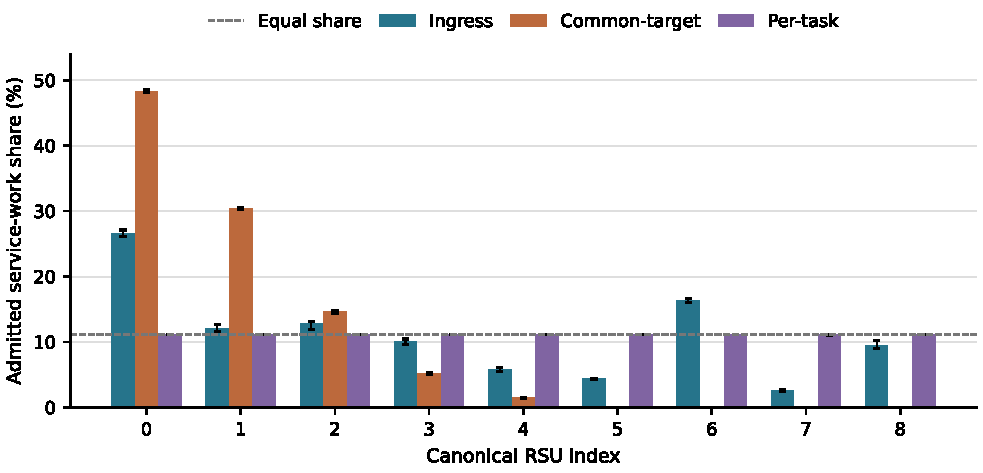
\includegraphics[width=\linewidth,height=.57\textheight,keepaspectratio]{assets/rsu_workload_distribution.pdf}
\caption[Morning RSU work distribution]{Admitted service-work distribution, redrawn from archived CSVs. Bars are means; whiskers are observed minima/maxima over four fleet draws, not confidence intervals. Aggregate shares motivated a separate post-hoc audit; they do not by themselves establish intermediate scheduling decisions or counterfactual task outcomes. Reading: compare the five occupied common-target destinations with the nearly even per-task distribution.}\label{fig:8}
\end{figure}
% END SOURCE BLOCK 300

% BEGIN SOURCE BLOCK 301 paragraph
The post-hoc audit found zero saved end-of-second workload and task counts in all four common-target runs, and target k at substep k whenever a V2I attempt exposed it. Empty substeps do not reveal the internal selector. Intermediate workloads were reconstructed, not saved directly, using recorded admissions/destinations and the qualified service reference. All endpoints and observable target minima agreed, although zero endpoints alone weakly constrain intermediate paths. Reconstructed pre-drain workload reached approximately 538.730 ms; task counts stayed below 26, far from the 1,000 ms drain and 6,220-task ceiling \hyperref[source-s9]{[S9]}.
% END SOURCE BLOCK 301

% BEGIN SOURCE BLOCK 302 paragraph
A conditional deduction from Algorithm~\ref{alg:1} explains the concentration. With $K$ substeps and $R$ RSUs, at most $\min(K,R)$ distinct destinations receive new assignments in one batch: each substep contributes at most one target, so their union has at most $K$ members. This bound does not require empty queues or a particular tie rule, and concerns new assignments rather than all work already present.
% END SOURCE BLOCK 302

% BEGIN SOURCE BLOCK 303 paragraph
A recurring low-index prefix additionally requires empty batch starts, positive productive admissions, lowest-index ties and no intervening drain. RSU 0 is selected first; its new work makes the next empty index preferable. Induction gives a prefix when $R\geq K$, while an unproductive substep does not advance it. End-of-batch clearing resets the tie. Without clearing or deterministic ties, the per-batch bound could hold while the full-run union covered every RSU.
% END SOURCE BLOCK 303

% BEGIN SOURCE BLOCK 304 paragraph
The arrays recorded 511,684 deadline-gate rejections and zero RSU-capacity rejections. In reconstructed states, every gate rejection coexisted with at least five idle RSUs possessing spare task capacity. Larger waiting rooms would not address that gate bottleneck. Spare capacity does not establish that each task would succeed elsewhere: redistribution changes later queues, and end-to-end latency also matters.
% END SOURCE BLOCK 304

% BEGIN SOURCE BLOCK 305 proof
\begin{proof}[Proof sketch]
Earlier-candidate dependence yields the unique causal solution and the candidate-count bound. The update reverses inclusion. Removing the first excess admission either exhausts capacity or fixes rejection of all later deadlines at or below its threshold. Every two replacements therefore eliminate at least one unresolved deadline class; one class needs one replacement. Appendix~\ref{app:C} gives the full induction and assumptions \hyperref[source-s14]{[S14]}.\end{proof}
% END SOURCE BLOCK 305

% BEGIN SOURCE BLOCK 306 paragraph
Here ``production'' means the studied evaluator configuration, not deployed roadside hardware. Its two deadline values imply three replacements suffice in exact arithmetic, including nonempty queues and capacity limits. The earlier three-threshold instability is outside this domain. This rules out unrestricted reconciliation failure as an exact-model explanation, while leaving target reselection and executable rounding distinct.
% END SOURCE BLOCK 306

% BEGIN SOURCE BLOCK 307 paragraph
The same model makes clearing structural from empty initialisation. The last admitted task sees less than 500 ms of backlog and contributes at most approximately 38.889 ms of service. Each queue therefore remains below 538.889 ms before a 1,000 ms drain. The observed zero endpoints and reconstructed maxima near 538 ms agree with this consequence. Queue clearing and the resulting destination prefix thus follow from the stated gate/service/timing assumptions, not traffic density alone. This deduction is conditional on exact admission arithmetic and service multiplier 1.
% END SOURCE BLOCK 307

% BEGIN SOURCE BLOCK 308 paragraph
Float32 limits executable equivalence. Inclusive prefix sums followed by subtraction can round differently from causal accumulation, changing a strict gate even for sub-0.001 ms differences. The completed numerical investigation includes discrete disagreements and a constructed alternating mask; that task misses its deadline under either treatment. These fixtures neither establish full-trajectory reachability nor measure historical prevalence. Appendix~\ref{app:C} retains the intermediate masks, threshold values and unsuccessful transfers, alongside the exact proof.
% END SOURCE BLOCK 308

% BEGIN SOURCE BLOCK 309 paragraph
Reselection can also lose completions. In the two-RSU illustration, both arms admit eight tasks; fixed-target admission completes eight and per-task reselection seven. Spreading earlier long-deadline work makes a later 100 ms task finish at 112.929 rather than 91.818 ms. Current workload omits future deadlines and the gate omits own service. Table~\ref{tab:C1} preserves the calculation: production task values, reduced infrastructure, zero transfers, and B replaying A targets rather than acting autonomously. Twelve transfers to the studied dimensions retained no loss. This identifies a possible interaction, not the cause or frequency of recorded losses; proposed full-evaluator prefixes remain unrun \hyperref[source-s10]{[S10]}, \hyperref[source-s14]{[S14]}.
% END SOURCE BLOCK 309

% BEGIN SOURCE BLOCK 310 paragraph
\textbf{Task outcomes in the original morning sample.}
% END SOURCE BLOCK 310

% BEGIN SOURCE BLOCK 311 paragraph
The mechanism explains destination concentration, but does not uniquely allocate the performance gap to individual decisions. The following recorded accounting locates gains and losses in the original four-draw morning comparison, separately from the eight-block confirmation.
% END SOURCE BLOCK 311

% BEGIN SOURCE BLOCK 312 paragraph
Table~\ref{tab:C2} partitions gains and losses over the same 1,744,116 offered tasks per original morning draw: 284,821 gains \ensuremath{-} 12,842 losses = 271,979 net successes. Previously gate-rejected tasks supply most gains, alongside recovered admitted misses; both kinds of losses remain visible. Later queues differ, so these are descriptive transitions, not individual-decision causal effects. The four draws remain the replications \hyperref[source-s13]{[S13]}, \hyperref[source-s14]{[S14]}.
% END SOURCE BLOCK 312

% BEGIN SOURCE BLOCK 313 table
\begingroup
\singlespacing\footnotesize\setlength{\tabcolsep}{3pt}
\begin{xltabular}{\textwidth}{@{}YYYYYY@{}}
\caption[Morning outcome accounting]{Morning ingress\ensuremath{\to}per-task outcome accounting, re-extracted from the authenticated paired results. Gains become successes; losses cease to be successes. All four primary draws are retained; the pilot is excluded. Reading: subtract losses from gains and check that the net equals the matched success difference.}\label{tab:C2} \\
\toprule
Seed & Gain: gate rejection & Gain: admitted miss & Loss: non-admitted & Loss: admitted miss & Net successes \\
\midrule\endfirsthead
\toprule
Seed & Gain: gate rejection & Gain: admitted miss & Loss: non-admitted & Loss: admitted miss & Net successes \\
\midrule\endhead
\bottomrule\endfoot
0 & 53,061 & 18,091 & 395 & 2,945 & 67,812 \\
2 & 64,418 & 19,125 & 496 & 4,144 & 78,903 \\
3 & 52,432 & 18,430 & 105 & 2,808 & 67,949 \\
4 & 41,823 & 17,441 & 48 & 1,901 & 57,315 \\
Total & 211,734 & 73,087 & 1,044 & 11,798 & 271,979 \\
\end{xltabular}
\endgroup
% END SOURCE BLOCK 313

% BEGIN SOURCE BLOCK 314 table
\begingroup
\singlespacing\footnotesize\setlength{\tabcolsep}{3pt}
\begin{xltabular}{\textwidth}{@{}YYYYYY@{}}
\caption[Type-level net changes]{Retrospective type-level net additional successes, per-task minus ingress. Each type has the stated offered population in every primary draw; full successes, admissions and failure counts are supplied in Appendix~\ref{app:D}. Reading: compare type-specific gains within each draw without treating types as additional independent replications.}\label{tab:C3} \\
\toprule
Type / deadline & Offered per draw & Seed 0 & Seed 2 & Seed 3 & Seed 4 \\
\midrule\endfirsthead
\toprule
Type / deadline & Offered per draw & Seed 0 & Seed 2 & Seed 3 & Seed 4 \\
\midrule\endhead
\bottomrule\endfoot
1 / 100 ms & 349,045 & +19,823 & +19,165 & +20,339 & +20,254 \\
2 / 500 ms & 523,060 & +72 & +62 & +6 & +5 \\
3 / 100 ms & 872,011 & +47,917 & +59,676 & +47,604 & +37,056 \\
\end{xltabular}
\endgroup
% END SOURCE BLOCK 314

% BEGIN SOURCE BLOCK 315 paragraph
Table~\ref{tab:C3} locates 79,581 net successes in Type 1, 145 in Type 2 and 192,253 in Type 3. Type 3 supplies 70.7\% of the net gain. Within-type improvements span 5.491--5.827, 0.001--0.014 and 4.249--6.843 points, respectively. The two 100 ms types differ substantially in payload and service (\S\,\ref{sec:2.3}). No type loses net successes in any draw, but individual losses persist. In draw 2, Type 1 gate rejections fall by 23,152 while admitted misses rise by 3,987. This supports reduced rejection as an important contributor, without isolating deadlines from communication/service demand or identifying individual-placement causal effects \hyperref[source-s15]{[S15]}.
% END SOURCE BLOCK 315

% BEGIN SOURCE BLOCK 316 heading
\appendixsection{app:D}{Type aggregation and engineering evidence}
% END SOURCE BLOCK 316

% BEGIN SOURCE BLOCK 317 paragraph
The retained retrospective type analysis read eight original primary-morning task arrays, authenticated their hashes, and aggregated categories by type; it was not repeated here. The prior 19-run admission validation and 23 task joins are reused, not repeated. All-task totals and paired net changes reconcile. The following table exposes every type/draw/arm; attainment uses the offered column. Other terminal failures are available in the linked CSV and unchanged within each pair.
% END SOURCE BLOCK 317

% BEGIN SOURCE BLOCK 318 table
\begingroup
\singlespacing\footnotesize\setlength{\tabcolsep}{3pt}
\begin{xltabular}{\textwidth}{@{}YYYYYYYY@{}}
\caption[Type outcomes]{Type outcomes. I = ingress, P = per-task; offered and category counts are tasks, attainment is percent. Gate rejection and admitted misses are disjoint. Reading: compare gate rejections, admitted misses and successes by task type under its own offered denominator.}\label{tab:D1} \\
\toprule
Seed / type & Arm & Offered & Success & Attainment & Admitted & Gate rejected & Admitted miss \\
\midrule\endfirsthead
\toprule
Seed / type & Arm & Offered & Success & Attainment & Admitted & Gate rejected & Admitted miss \\
\midrule\endhead
\bottomrule\endfoot
0/1 & I & 349,045 & 252,283 & 72.278 & 328,923 & 19,548 & 76,640 \\
0/1 & P & 349,045 & 272,106 & 77.957 & 347,605 & 866 & 75,499 \\
0/2 & I & 523,060 & 516,034 & 98.657 & 522,134 & 46 & 6,100 \\
0/2 & P & 523,060 & 516,106 & 98.671 & 522,180 & 0 & 6,074 \\
0/3 & I & 872,011 & 780,747 & 89.534 & 821,868 & 48,572 & 41,121 \\
0/3 & P & 872,011 & 828,664 & 95.029 & 868,284 & 2,156 & 39,620 \\
2/1 & I & 349,045 & 242,629 & 69.512 & 324,165 & 24,149 & 81,536 \\
2/1 & P & 349,045 & 261,794 & 75.003 & 347,317 & 997 & 85,523 \\
2/2 & I & 523,060 & 515,409 & 98.537 & 521,901 & 40 & 6,492 \\
2/2 & P & 523,060 & 515,471 & 98.549 & 521,941 & 0 & 6,470 \\
2/3 & I & 872,011 & 768,687 & 88.151 & 809,915 & 60,362 & 41,228 \\
2/3 & P & 872,011 & 828,363 & 94.995 & 867,771 & 2,506 & 39,408 \\
3/1 & I & 349,045 & 253,921 & 72.747 & 330,364 & 18,383 & 76,443 \\
3/1 & P & 349,045 & 274,260 & 78.574 & 348,537 & 210 & 74,277 \\
3/2 & I & 523,060 & 517,080 & 98.857 & 522,533 & 1 & 5,453 \\
3/2 & P & 523,060 & 517,086 & 98.858 & 522,534 & 0 & 5,448 \\
3/3 & I & 872,011 & 782,701 & 89.758 & 824,760 & 46,357 & 42,059 \\
3/3 & P & 872,011 & 830,305 & 95.217 & 870,539 & 578 & 40,234 \\
4/1 & I & 349,045 & 260,449 & 74.618 & 333,800 & 14,596 & 73,351 \\
4/1 & P & 349,045 & 280,703 & 80.420 & 348,250 & 146 & 67,547 \\
4/2 & I & 523,060 & 516,064 & 98.662 & 521,928 & 1 & 5,864 \\
4/2 & P & 523,060 & 516,069 & 98.663 & 521,929 & 0 & 5,860 \\
4/3 & I & 872,011 & 795,155 & 91.186 & 834,388 & 35,739 & 39,233 \\
4/3 & P & 872,011 & 832,211 & 95.436 & 869,818 & 309 & 37,607 \\
\end{xltabular}
\endgroup
% END SOURCE BLOCK 318

% BEGIN SOURCE BLOCK 319 paragraph
The \href{\detokenize{../empirical_extension_2026-09-08/analysis/results/BENCHMARK.json}}{benchmark record} retains lowering/compilation times, median, quartiles, p95, minima/maxima, compiler buffer estimates and exact source/runtime identities for all 16 configurations. \href{\detokenize{../empirical_extension_2026-09-08/analysis/results/BENCHMARK_TIMES.csv}}{Raw call durations} permit descriptive timing checks. \href{\detokenize{../empirical_extension_2026-09-08/confirmation/PRECISION.json}}{Precision sensitivity} records pre-outcome assumptions about block variance; it is not observed power for the new results.
% END SOURCE BLOCK 319

% BEGIN SOURCE BLOCK 320 heading
\appendixsection{app:E}{Joint-randomness study controls and execution}
% END SOURCE BLOCK 320

% BEGIN SOURCE BLOCK 321 paragraph
The execution-authorised seal preserves the disabled preparation package and binds its own source version, current actor/trace identities, runtime, output root, lock and qualification receipts. Fleet/evaluator pairs are (100,200) through (107,207). The accessible manifest check found no prior outcomes for these pairs; this is a scoped absence check, not proof that no record exists elsewhere. Block 0 starts ingress/common-target/per-task/round-robin; each subsequent block rotates that order by one position.
% END SOURCE BLOCK 321

% BEGIN SOURCE BLOCK 322 paragraph
Qualification used the previously inspected fleet/evaluator pair (1,0), never confirmation outcomes. Three frozen/instrumented pairs ran for 300 steps, followed by round-robin at 300 and a fresh-process 150-step restart: eight attempts total. All 83 shared scientific fields matched exactly in each unchanged-arm pair. The 300-step cyclic run advanced its pointer 8,817 times, including 28 subsequently rejected attempts; its final pointer was 6. The 150-step run matched the longer run's prefix. No unavailable-radio, RSU-capacity or local-capacity failures occurred in these short records, so their end-to-end branches were not empirically exercised. Preserved kernel tests cover those branches separately. Qualification is neither an extra replication nor proof of full-horizon equivalence.
% END SOURCE BLOCK 322

% BEGIN SOURCE BLOCK 323 paragraph
Added records expose final admission independently of success, actual local/peer service, queue counts, post-service workloads, SoC/energy and cyclic pointer state. Negative checks refused a corrupted offered count, mismatched shared-input binding, absent block receipt and changed output hash. A separate prelaunch critique identified a possible alternate-root attempt-budget bypass, incomplete type-summary checking and misleading failed-process timing. The final version binds one raw root/global lock, validates type numerators/denominators and records failure phase and elapsed process time. Existing short records were rechecked; no ninth qualification evaluator ran.
% END SOURCE BLOCK 323

% BEGIN SOURCE BLOCK 324 paragraph
Each full cell requires exact discrete accounting, proposal/admission/execution/forwarding consistency, penalty latency exactly ten times the deadline, inclusive deadline success and independent queue-work reconstruction. Retained tolerances are 0.01 ms absolute per queue-second for service conservation, 0.001 ms plus relative 0.000001 for drain, and 0.000001 task for reconstructed JSON score/type numerators. Within each block, fleet arrays, key streams, offers, observation descriptors, operational types/sizes and pre-admission service work must agree exactly. Observations, logits, actions, SoC and selected radio quantities are separately reported; equality is not forced.
% END SOURCE BLOCK 324

% BEGIN SOURCE BLOCK 325 paragraph
Execution is serial with at most 32 full attempts including failures, no retries or seed substitution, a three-hour per-cell timeout, 50 GiB initial free-space requirement and 20 GiB before each attempt. Incomplete attempts are retained. Completed-output hashes, commands, source identities and all eight block receipts gate the sealed primary analysis. The first included block supplies a remaining-runtime estimate; effects cannot change continuation. Process time includes startup, compilation, evaluation and compressed output writing; validation is timed separately. These times are not the scheduler-only benchmark in Table~\ref{tab:8}.
% END SOURCE BLOCK 325

% BEGIN SOURCE BLOCK 326 paragraph
The completed full matrix has 32 valid cells, eight valid block receipts and no failed attempts. The following tables retain every cell and block. I = ingress, $D$ = common-target, P = per-task and $R$ = round-robin; fleet/evaluator seeds are 100+$b$ and 200+$b$ for block b. Other terminal categories are retained in CELL\_RESULTS.csv and each validation receipt.
% END SOURCE BLOCK 326

% BEGIN SOURCE BLOCK 327 table
\begingroup
\singlespacing\footnotesize\setlength{\tabcolsep}{3pt}
\begin{xltabular}{\textwidth}{@{}YYYYYYY@{}}
\caption[All confirmation cells]{Full new-study counts. Offered populations match within blocks; attainment is offered-task percent. Gate rejection and admitted misses are disjoint. Reading: retain all eight paired blocks and four policies rather than pooling tasks as replications.}\label{tab:E1} \\
\toprule
Block / arm & Offered & Admitted & Successes & Attainment & Gate rejected & Admitted misses \\
\midrule\endfirsthead
\toprule
Block / arm & Offered & Admitted & Successes & Attainment & Gate rejected & Admitted misses \\
\midrule\endhead
\bottomrule\endfoot
0/I & 1,744,761 & 1,655,779 & 1,525,913 & 87.457 & 86,625 & 129,866 \\
0/$D$ & 1,744,761 & 1,582,636 & 1,459,384 & 83.644 & 159,768 & 123,252 \\
0/P & 1,744,761 & 1,737,398 & 1,605,152 & 91.998 & 5,006 & 132,246 \\
0/$R$ & 1,744,761 & 1,726,560 & 1,592,830 & 91.292 & 15,844 & 133,730 \\
1/I & 1,740,970 & 1,662,805 & 1,534,040 & 88.114 & 76,351 & 128,765 \\
1/$D$ & 1,740,970 & 1,593,599 & 1,470,819 & 84.483 & 145,557 & 122,780 \\
1/P & 1,740,970 & 1,736,301 & 1,607,919 & 92.358 & 2,855 & 128,382 \\
1/$R$ & 1,740,970 & 1,727,104 & 1,596,377 & 91.695 & 12,052 & 130,727 \\
2/I & 1,741,855 & 1,639,136 & 1,510,719 & 86.730 & 99,922 & 128,417 \\
2/$D$ & 1,741,855 & 1,556,771 & 1,436,166 & 82.450 & 182,287 & 120,605 \\
2/P & 1,741,855 & 1,732,694 & 1,598,164 & 91.751 & 6,364 & 134,530 \\
2/$R$ & 1,741,855 & 1,718,789 & 1,583,772 & 90.924 & 20,269 & 135,017 \\
3/I & 1,744,227 & 1,677,045 & 1,557,192 & 89.277 & 65,368 & 119,853 \\
3/$D$ & 1,744,227 & 1,616,965 & 1,501,691 & 86.095 & 125,448 & 115,274 \\
3/P & 1,744,227 & 1,740,631 & 1,624,157 & 93.116 & 1,782 & 116,474 \\
3/$R$ & 1,744,227 & 1,734,468 & 1,614,712 & 92.575 & 7,945 & 119,756 \\
4/I & 1,743,484 & 1,680,263 & 1,560,221 & 89.489 & 61,226 & 120,042 \\
4/$D$ & 1,743,484 & 1,623,533 & 1,507,624 & 86.472 & 117,956 & 115,909 \\
4/P & 1,743,484 & 1,738,717 & 1,622,888 & 93.083 & 2,772 & 115,829 \\
4/$R$ & 1,743,484 & 1,732,685 & 1,613,895 & 92.567 & 8,804 & 118,790 \\
5/I & 1,745,078 & 1,685,944 & 1,564,006 & 89.624 & 56,788 & 121,938 \\
5/$D$ & 1,745,078 & 1,629,177 & 1,511,177 & 86.597 & 113,555 & 118,000 \\
5/P & 1,745,078 & 1,740,768 & 1,623,996 & 93.062 & 1,964 & 116,772 \\
5/$R$ & 1,745,078 & 1,735,213 & 1,614,934 & 92.542 & 7,519 & 120,279 \\
6/I & 1,742,095 & 1,669,339 & 1,541,879 & 88.507 & 69,142 & 127,460 \\
6/$D$ & 1,742,095 & 1,603,847 & 1,481,655 & 85.050 & 134,634 & 122,192 \\
6/P & 1,742,095 & 1,736,400 & 1,611,494 & 92.503 & 2,081 & 124,906 \\
6/$R$ & 1,742,095 & 1,729,087 & 1,601,138 & 91.909 & 9,394 & 127,949 \\
7/I & 1,744,742 & 1,657,846 & 1,531,566 & 87.782 & 84,523 & 126,280 \\
7/$D$ & 1,744,742 & 1,588,286 & 1,468,334 & 84.158 & 154,083 & 119,952 \\
7/P & 1,744,742 & 1,736,713 & 1,608,728 & 92.204 & 5,656 & 127,985 \\
7/$R$ & 1,744,742 & 1,726,431 & 1,596,904 & 91.527 & 15,938 & 129,527 \\
\end{xltabular}
\endgroup
% END SOURCE BLOCK 327

% BEGIN SOURCE BLOCK 328 table
\begingroup
\singlespacing\footnotesize\setlength{\tabcolsep}{3pt}
\begin{xltabular}{\textwidth}{@{}YYYY@{}}
\caption[Eight paired effects]{All eight paired effects, percentage points. These blocks, not tasks or RSUs, are the new replications. Reading: compare the three paired arm differences within each joint block; eight blocks define the replication unit.}\label{tab:E2} \\
\toprule
Block & Per-task \ensuremath{-} ingress & Common-target \ensuremath{-} ingress & Per-task \ensuremath{-} round-robin \\
\midrule\endfirsthead
\toprule
Block & Per-task \ensuremath{-} ingress & Common-target \ensuremath{-} ingress & Per-task \ensuremath{-} round-robin \\
\midrule\endhead
\bottomrule\endfoot
0 & +4.542 & \ensuremath{-}3.813 & +0.706 \\
1 & +4.244 & \ensuremath{-}3.631 & +0.663 \\
2 & +5.020 & \ensuremath{-}4.280 & +0.826 \\
3 & +3.839 & \ensuremath{-}3.182 & +0.542 \\
4 & +3.594 & \ensuremath{-}3.017 & +0.516 \\
5 & +3.438 & \ensuremath{-}3.027 & +0.519 \\
6 & +3.996 & \ensuremath{-}3.457 & +0.594 \\
7 & +4.423 & \ensuremath{-}3.624 & +0.678 \\
\end{xltabular}
\endgroup
% END SOURCE BLOCK 328

% BEGIN SOURCE BLOCK 329 paragraph
Actions matched exactly in all 24 non-reference arm/block comparisons. Small observation and logit differences occurred in block 1; they did not change actions. The estimand remains the total scheduling intervention under frozen weights. Observed action matching extends the original finding to these streams without forcing replay or guaranteeing future equality. In block 1 (fleet 101/evaluator 201), each alternative differed from ingress by at most 0.0000000149012 in observations and SoC, and 0.000000357628 in logits. These are dimensionless recorded differences; no action was altered or forced. The \href{\detokenize{../joint_confirmation_2026-09-08/evidence/BLOCK_CONTROLS.json}}{block receipts} retain every comparison and exact maxima. The \href{\detokenize{../joint_confirmation_2026-09-08/evidence/CELL_RESULTS.json}}{cell records} and \href{\detokenize{../joint_confirmation_2026-09-08/evidence/PAIRED_EFFECTS.csv}}{paired effects} preserve unrounded values. No task-level significance tests or new type subgroup analysis were added.
% END SOURCE BLOCK 329

% BEGIN SOURCE BLOCK 330 paragraph
All 32 records passed final-admission/score/category/penalty, assignment and queue checks under the sealed contract. Maximum reconstructed per-queue-second service discrepancy was 0.000121593 ms for RSUs and 0.000244141 ms for vehicle queues. This finite result does not certify every possible path or repair the historical off scorer.
% END SOURCE BLOCK 330

% BEGIN SOURCE BLOCK 331 paragraph
The campaign elapsed 6440.25 seconds (107.34 minutes) from first attempt to completion. Full evaluator processes took 6375.54 seconds in total; cell validation took 49.59 seconds, block validation 10.83 seconds, and sealed analysis with completion/hash checks 3.44 seconds. Qualification processes separately took 68.09 seconds. \href{\detokenize{../joint_confirmation_2026-09-08/evidence/TIMING.json}}{Timing records} and per-cell logs retain the exact boundaries. The first-block estimate used runtime only.
% END SOURCE BLOCK 331

% BEGIN SOURCE BLOCK 332 paragraph
The \href{\detokenize{../joint_confirmation_2026-09-08/evidence/RAW_INVENTORY.json}}{raw inventory} binds the locally retained task/step arrays and supporting files. The \href{\detokenize{../joint_confirmation_2026-09-08/document/verify_results.py}}{verifier (requires NumPy and SciPy)} regenerates central tables from compact evidence and accepts an optional explicit raw root for integrity checking. Compact arithmetic is not repeated task-level validation; hashes are not a backup. Approved off-machine storage and examiner access remain unresolved.
% END SOURCE BLOCK 332

\end{document}
